\documentclass[12pt,oneside]{paper}

\usepackage{listings}
\renewcommand{\lstlistingname}{saucecode}

% タイトル
\title{安定飛行ができるドローンの開発}
\author{天王地亮太}

\begin{document}
% 行間
\setlength{\baselineskip}{9truemm}

%文字間
\kanjiskip=.53zw plus 3pt minus 3pt
\xkanjiskip=.53zw plus 3pt minus 3pt

% 目次
\tableofcontents
%\newpage

% 本文

\chapter{序論}
\section{研究の背景}
現在,図\ref{fig:doron}のようなドローンは物資輸送,それぞれが自作した物でスポーツ・レースを行ったり,空から農薬を撒くなどの農業,果ては火山の火口や災害などで人が立ち入れない所の調査など,幅広く利用されている.

本年は,自作したドローンで飛行ロボットコンテストという室内飛行機の大会に出場しようと試みた.
飛行ロボットコンテストとは,2006年から開催された日本航空宇宙学会が主催の室内飛行用航空機型ロボットによる競技.自作ドローンが参加可能な,マルチコプタ部門は2015年の第11回から登場した.

\begin{figure}[htbp]
  \begin{center}
    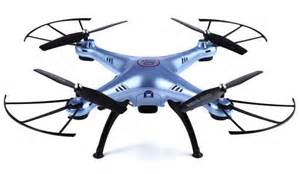
\includegraphics[width=100mm]{ga/doron.jpg}
    \end{center}
  \caption{ドローン}
 \label{fig:doron}
\end{figure}

\section{研究の目的}
ドローンの製作に必要なプログラムと制御に関する知識がなく,結果大会のエントリーの締切までに作り上げることができず,参加すること事態できなかった.そこで製作に関わる制御の知識をドローンを製作しながら学んでいき,ドローンが外部からの突然加わる力によって傾き墜落しないような安定飛行ができる機体の製作を目標とする.



\section{論文の構成}
この論文では以下のように構成されている.
1章では,我々の研究目的やドローンの原理について説明したものである.


2章では,ドローンのフレームを設計製作に関するものである.


3章では,使用する電子部品,センサー,マイコンの機能を説明したものである.


4章では,センサーとマイコン間の通信方法を記す.


5章では,ドローンの全体の制御の流れや,センサーからのデータを処理し本体の制御に反映する方法を記す.


6章では,前章の方法で得た結果を記す.


7章では,本研究において大きな力となった関係者各員に謝辞を記す.
\chapter{フレームの設計製作}

\section{ドローンの飛行原理}
ドローンは4~8枚ほどのプロペラが同時に回転して飛びますが,図\ref{fig:gen}のように右上のプロペラは右回転,左上のプロペラは左回転と,隣り合うプロペラとは逆回転をしている.これにより,本体が回転しようとするチカラを相殺して,飛行が可能になっている.

\begin{figure}[H]
  \begin{center}
    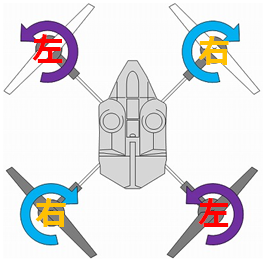
\includegraphics[width=70mm]{ga/gen.png}
    \end{center}
  \caption{ドローンのプロペラ回転方向}
 \label{fig:gen}
\end{figure}

前進をする場合は,図\ref{fig:zen}のように進みたい方向のプロペラの回転数を遅くし,その反対のプロペラの回転数を速くすることで,前進を行う.又,後退ならばその反対のことをすることで後退する.

\begin{figure}[H]
  \begin{center}
    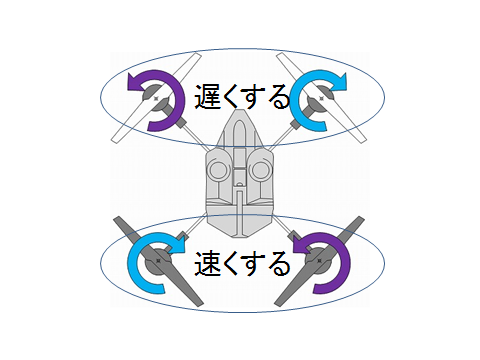
\includegraphics[width=100mm]{ga/zen.png}
    \end{center}
  \caption{ドローンを前に進ませるとき}
 \label{fig:zen}
\end{figure}

右に移動する場合は,図\ref{fig:rig}のように右側のプロペラの回転数が遅く,左側のプロペラの回転数が速くします.又,左に移動する場合もこの方法と反対のことをすればよい.

\begin{figure}[H]
  \begin{center}
    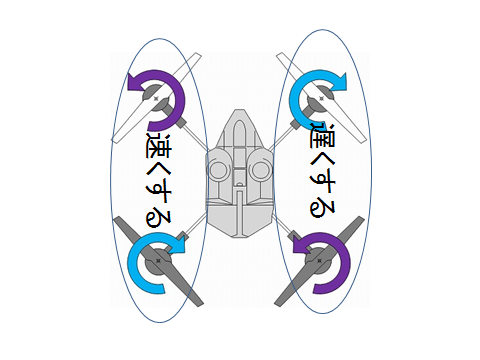
\includegraphics[width=100mm]{ga/rig.png}
    \end{center}
  \caption{ドローンを右へ移動するとき}
 \label{fig:rig}
\end{figure}

左回転をする場合は,図\ref{fig:rol}のように右前のプロペラと左後ろのプロペラの回転数が速く,左前のプロペラと右後ろのプロペラの回転数が遅くする.又,右に移動する場合もこの方法と反対のことをすればよい.

\begin{figure}[H]
  \begin{center}
    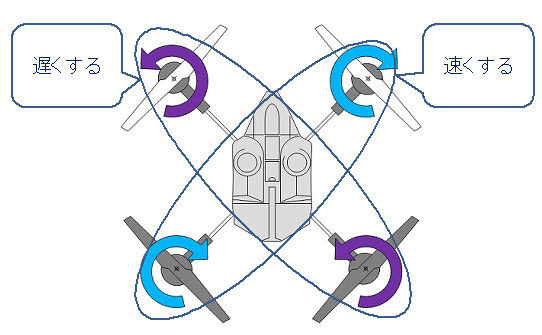
\includegraphics[width=100mm]{ga/rol.png}
    \end{center}
  \caption{ドローンを左回転させるとき}
 \label{fig:rol}
\end{figure}


\section{設計}始めにインターネット等で図\ref{fig:sihan}のような市販のドローンを調べた.

\begin{figure}[H]
  \begin{center}
    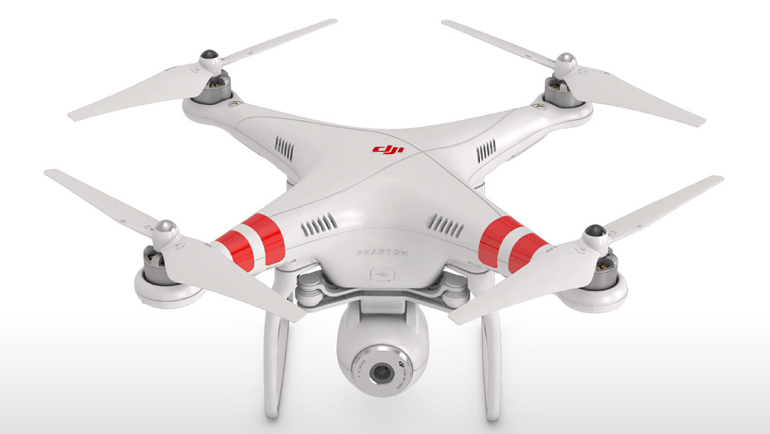
\includegraphics[width=100mm]{ga/doron3.png}
    \end{center}
  \caption{市販品例}
 \label{fig:sihan}
\end{figure}

それをもとにして形だけを作り出したものが図\ref{fig:ori}のフレームとなり,ここから軽量化をコンセプトとし電子部品を含め総重量300g以下を目指し改良を続け製作を行ってきた.
なお,フレームの材料は厚さ2mmのベニヤ板を使用している.

\begin{figure}[H]
  \begin{center}
    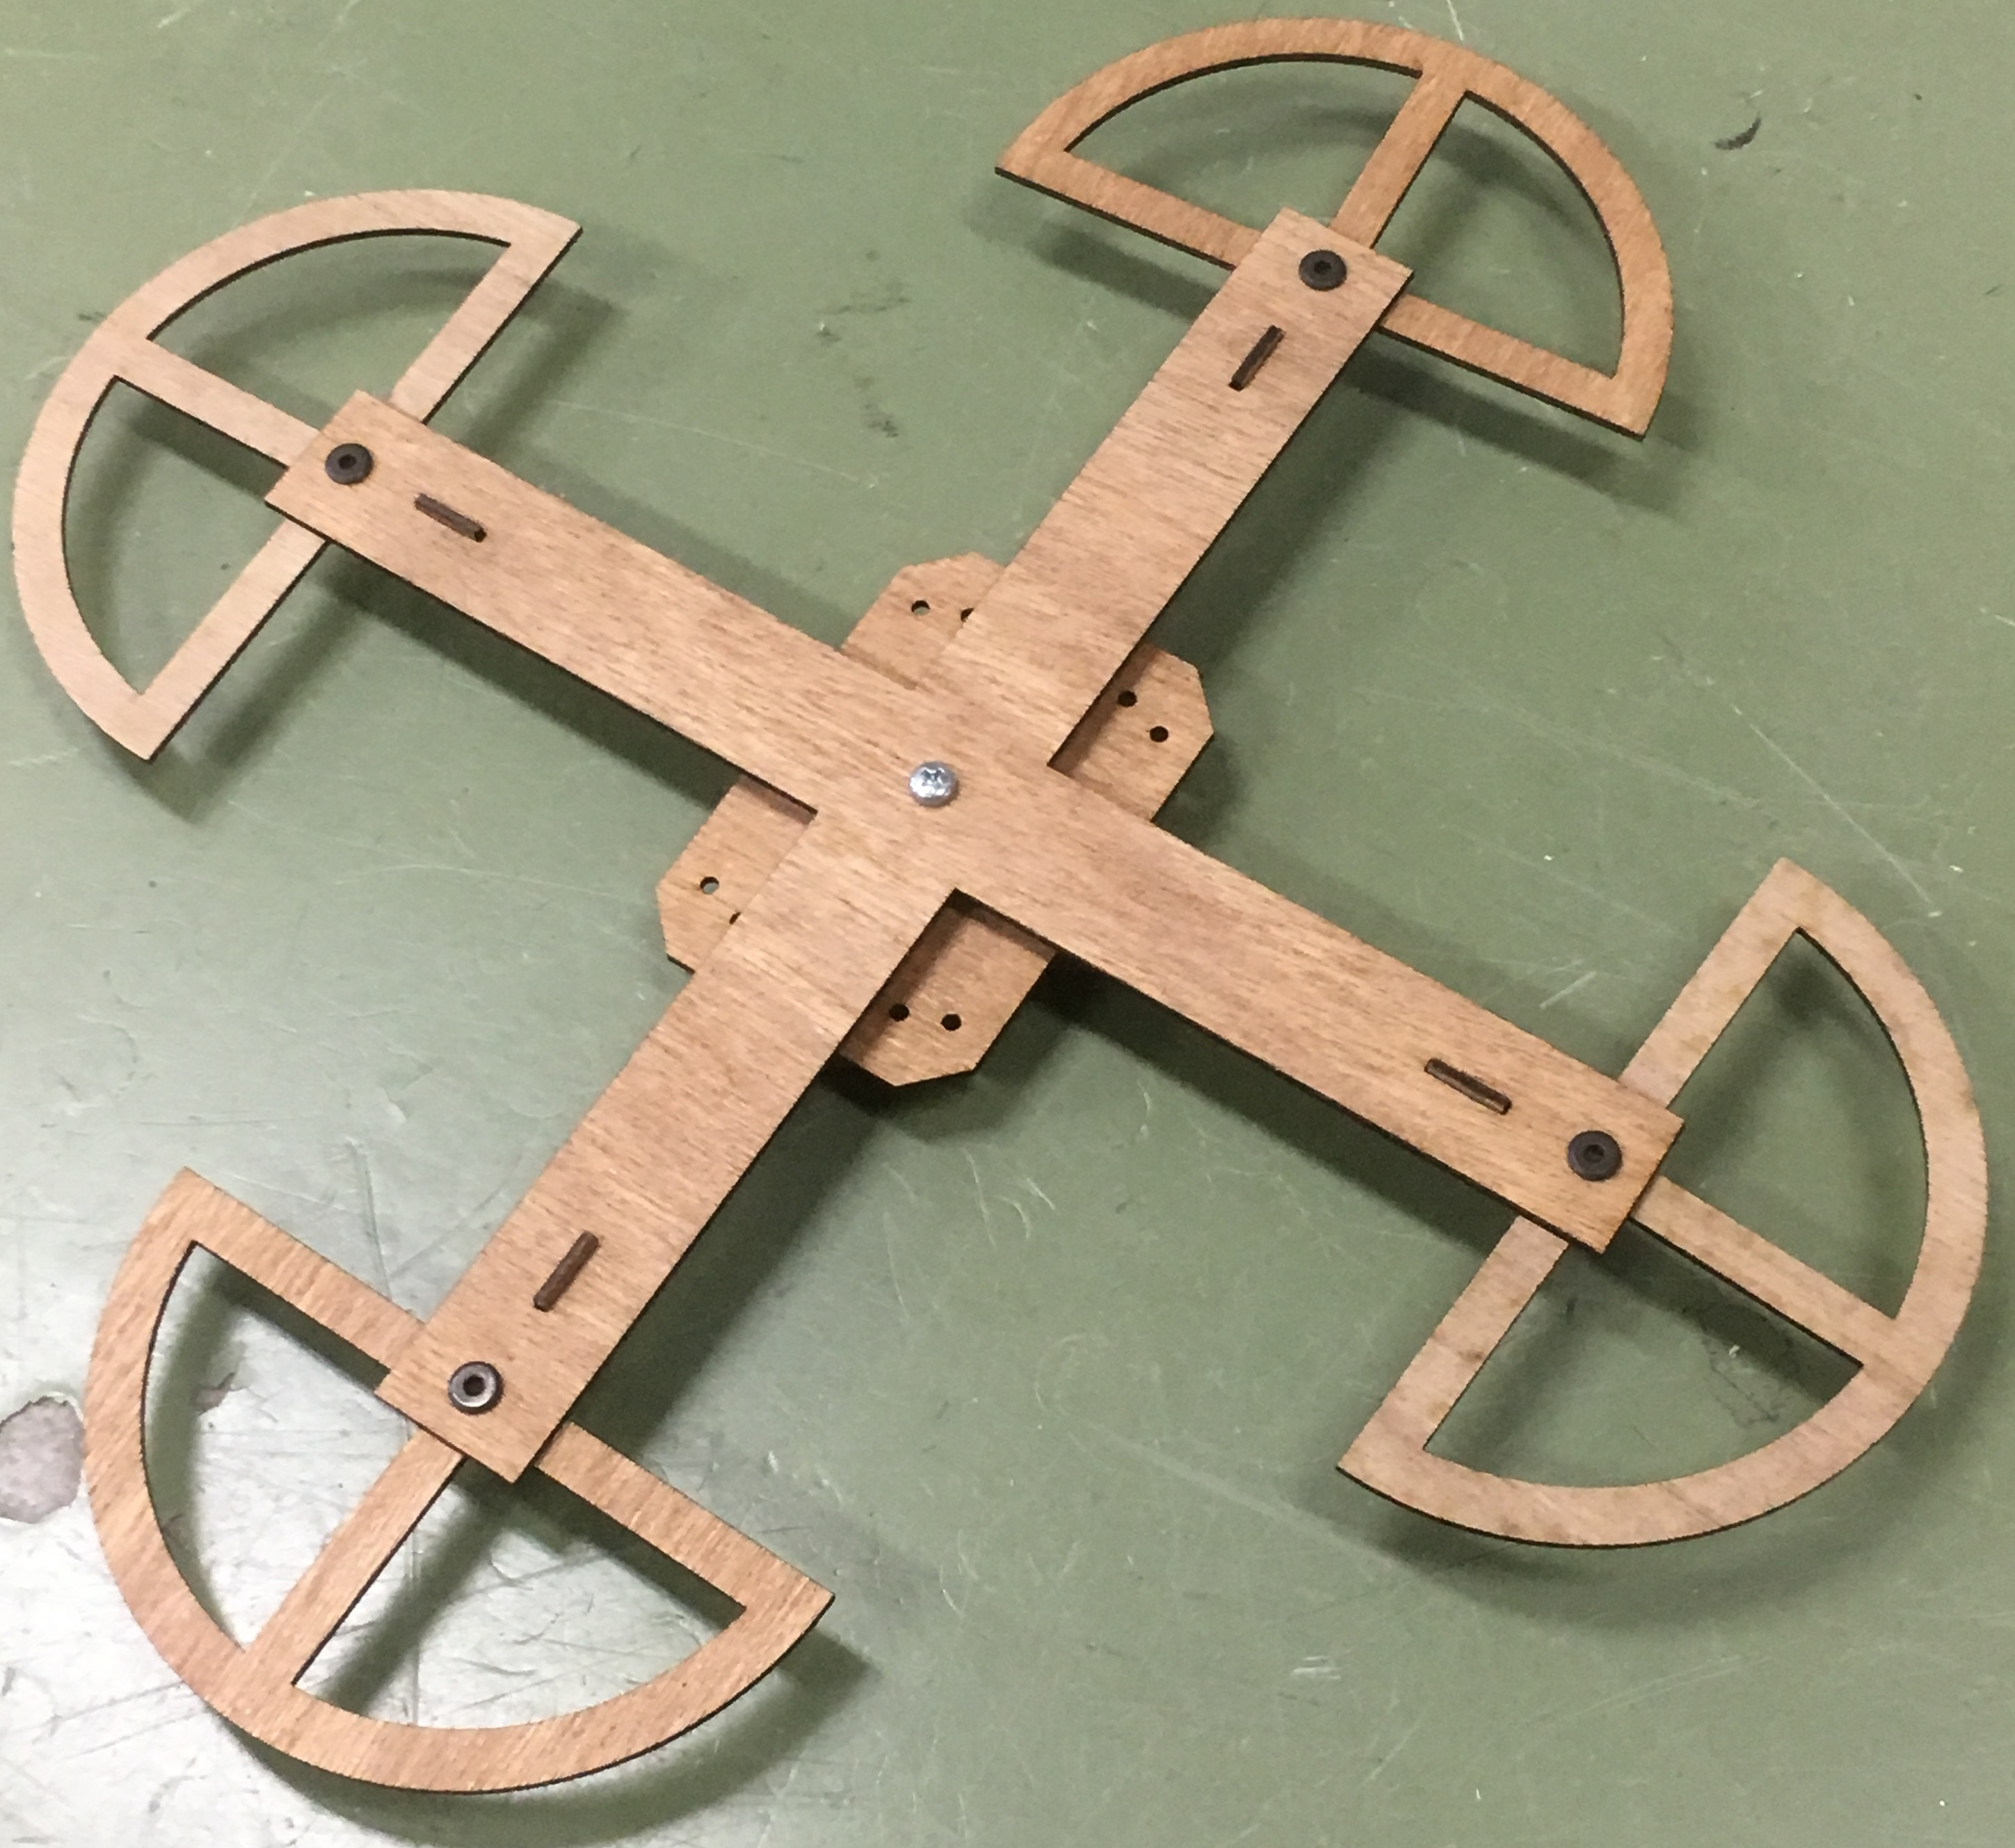
\includegraphics[width=100mm]{ga/ori.jpg}
    \end{center}
  \caption{フレーム初期案}
 \label{fig:ori}
\end{figure}

この初期案はとにかく不格好で,重量もフレームだけで80g以上もあった.
ここでの改良は,腕や土台,プロペラガードを一つのパーツとし,パーツの接合をねじ等にするとその分重量が増量してしまうので各パーツの接合部をはめ合いに,接着剤で接着可能なものとした.
さらにフレームの所々にトラス構造のような穴をあけ,軽量化とともに剛性も上げた.

\begin{figure}[H]
  \begin{center}
    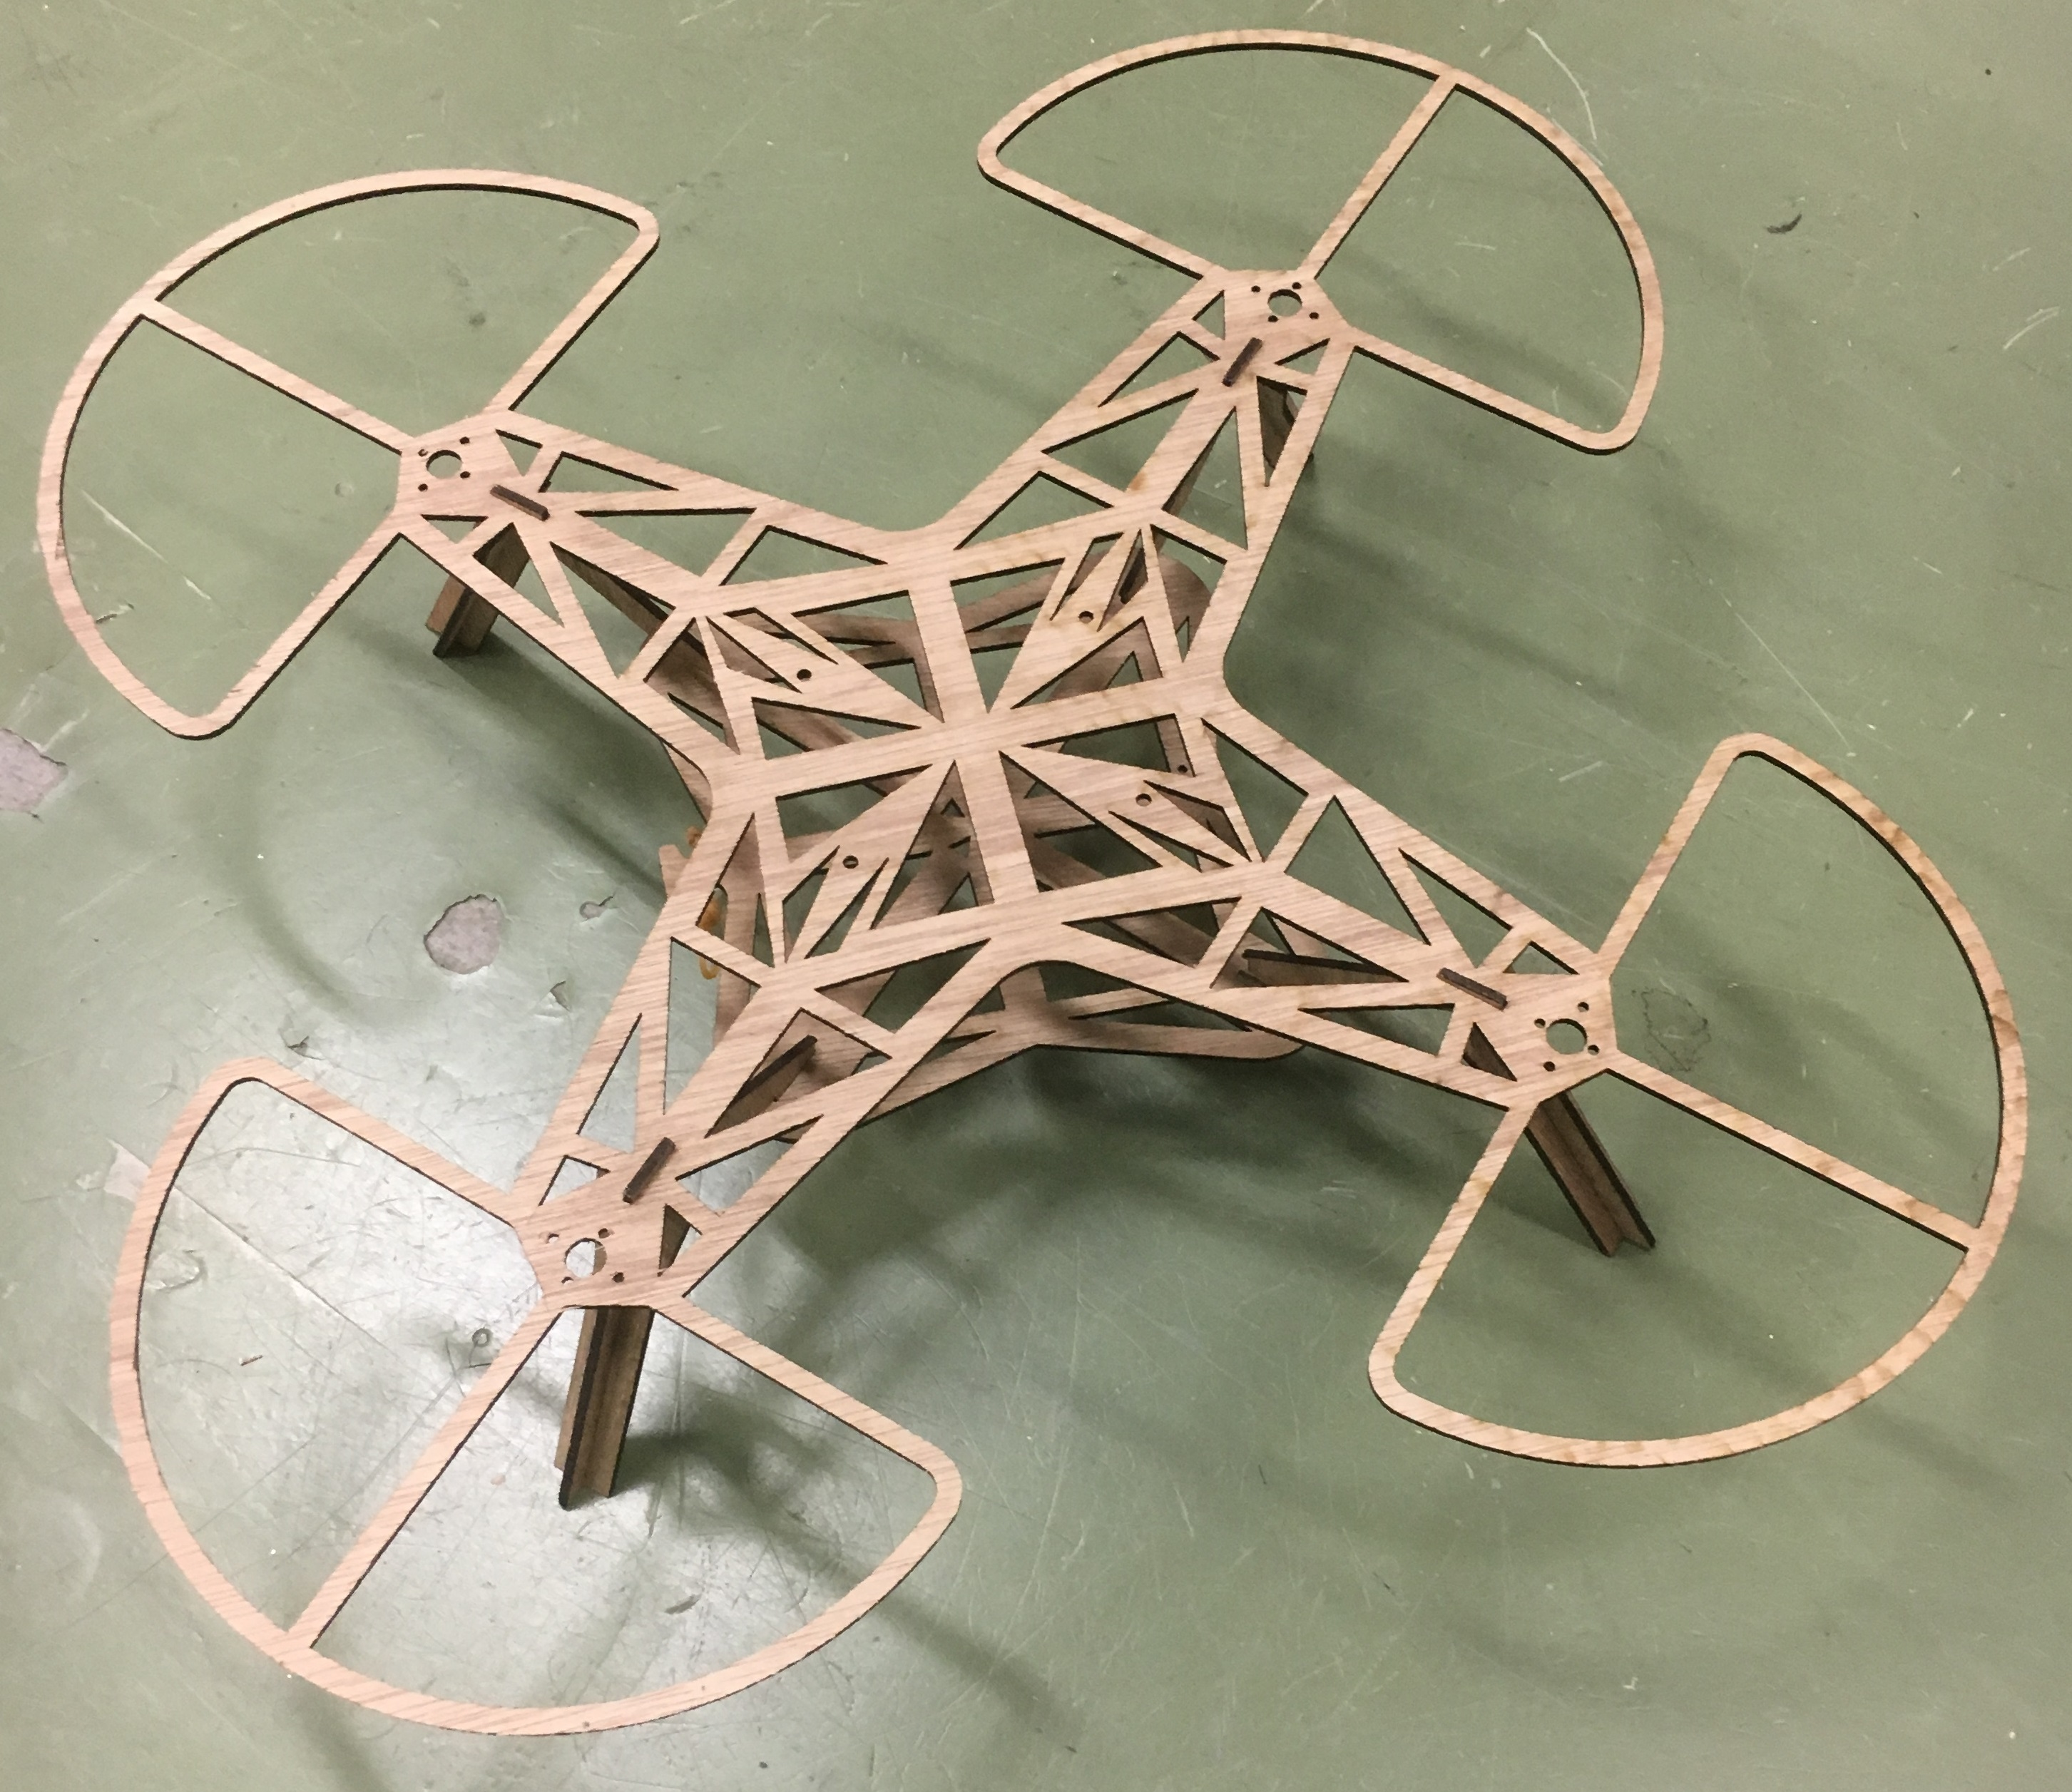
\includegraphics[width=100mm]{ga/sec.jpg}
    \end{center}
  \caption{改良その1}
 \label{fig:sec}
\end{figure}

ここからトラス構造の剛性を失わずにどれだけ開けた穴を広げられるか,他の開け方ではどれだけ軽量化を図れるかを実際に製作し重量を測定した.
なお,この時点の重量は70g前後.

\begin{figure}[H]
  \begin{center}
    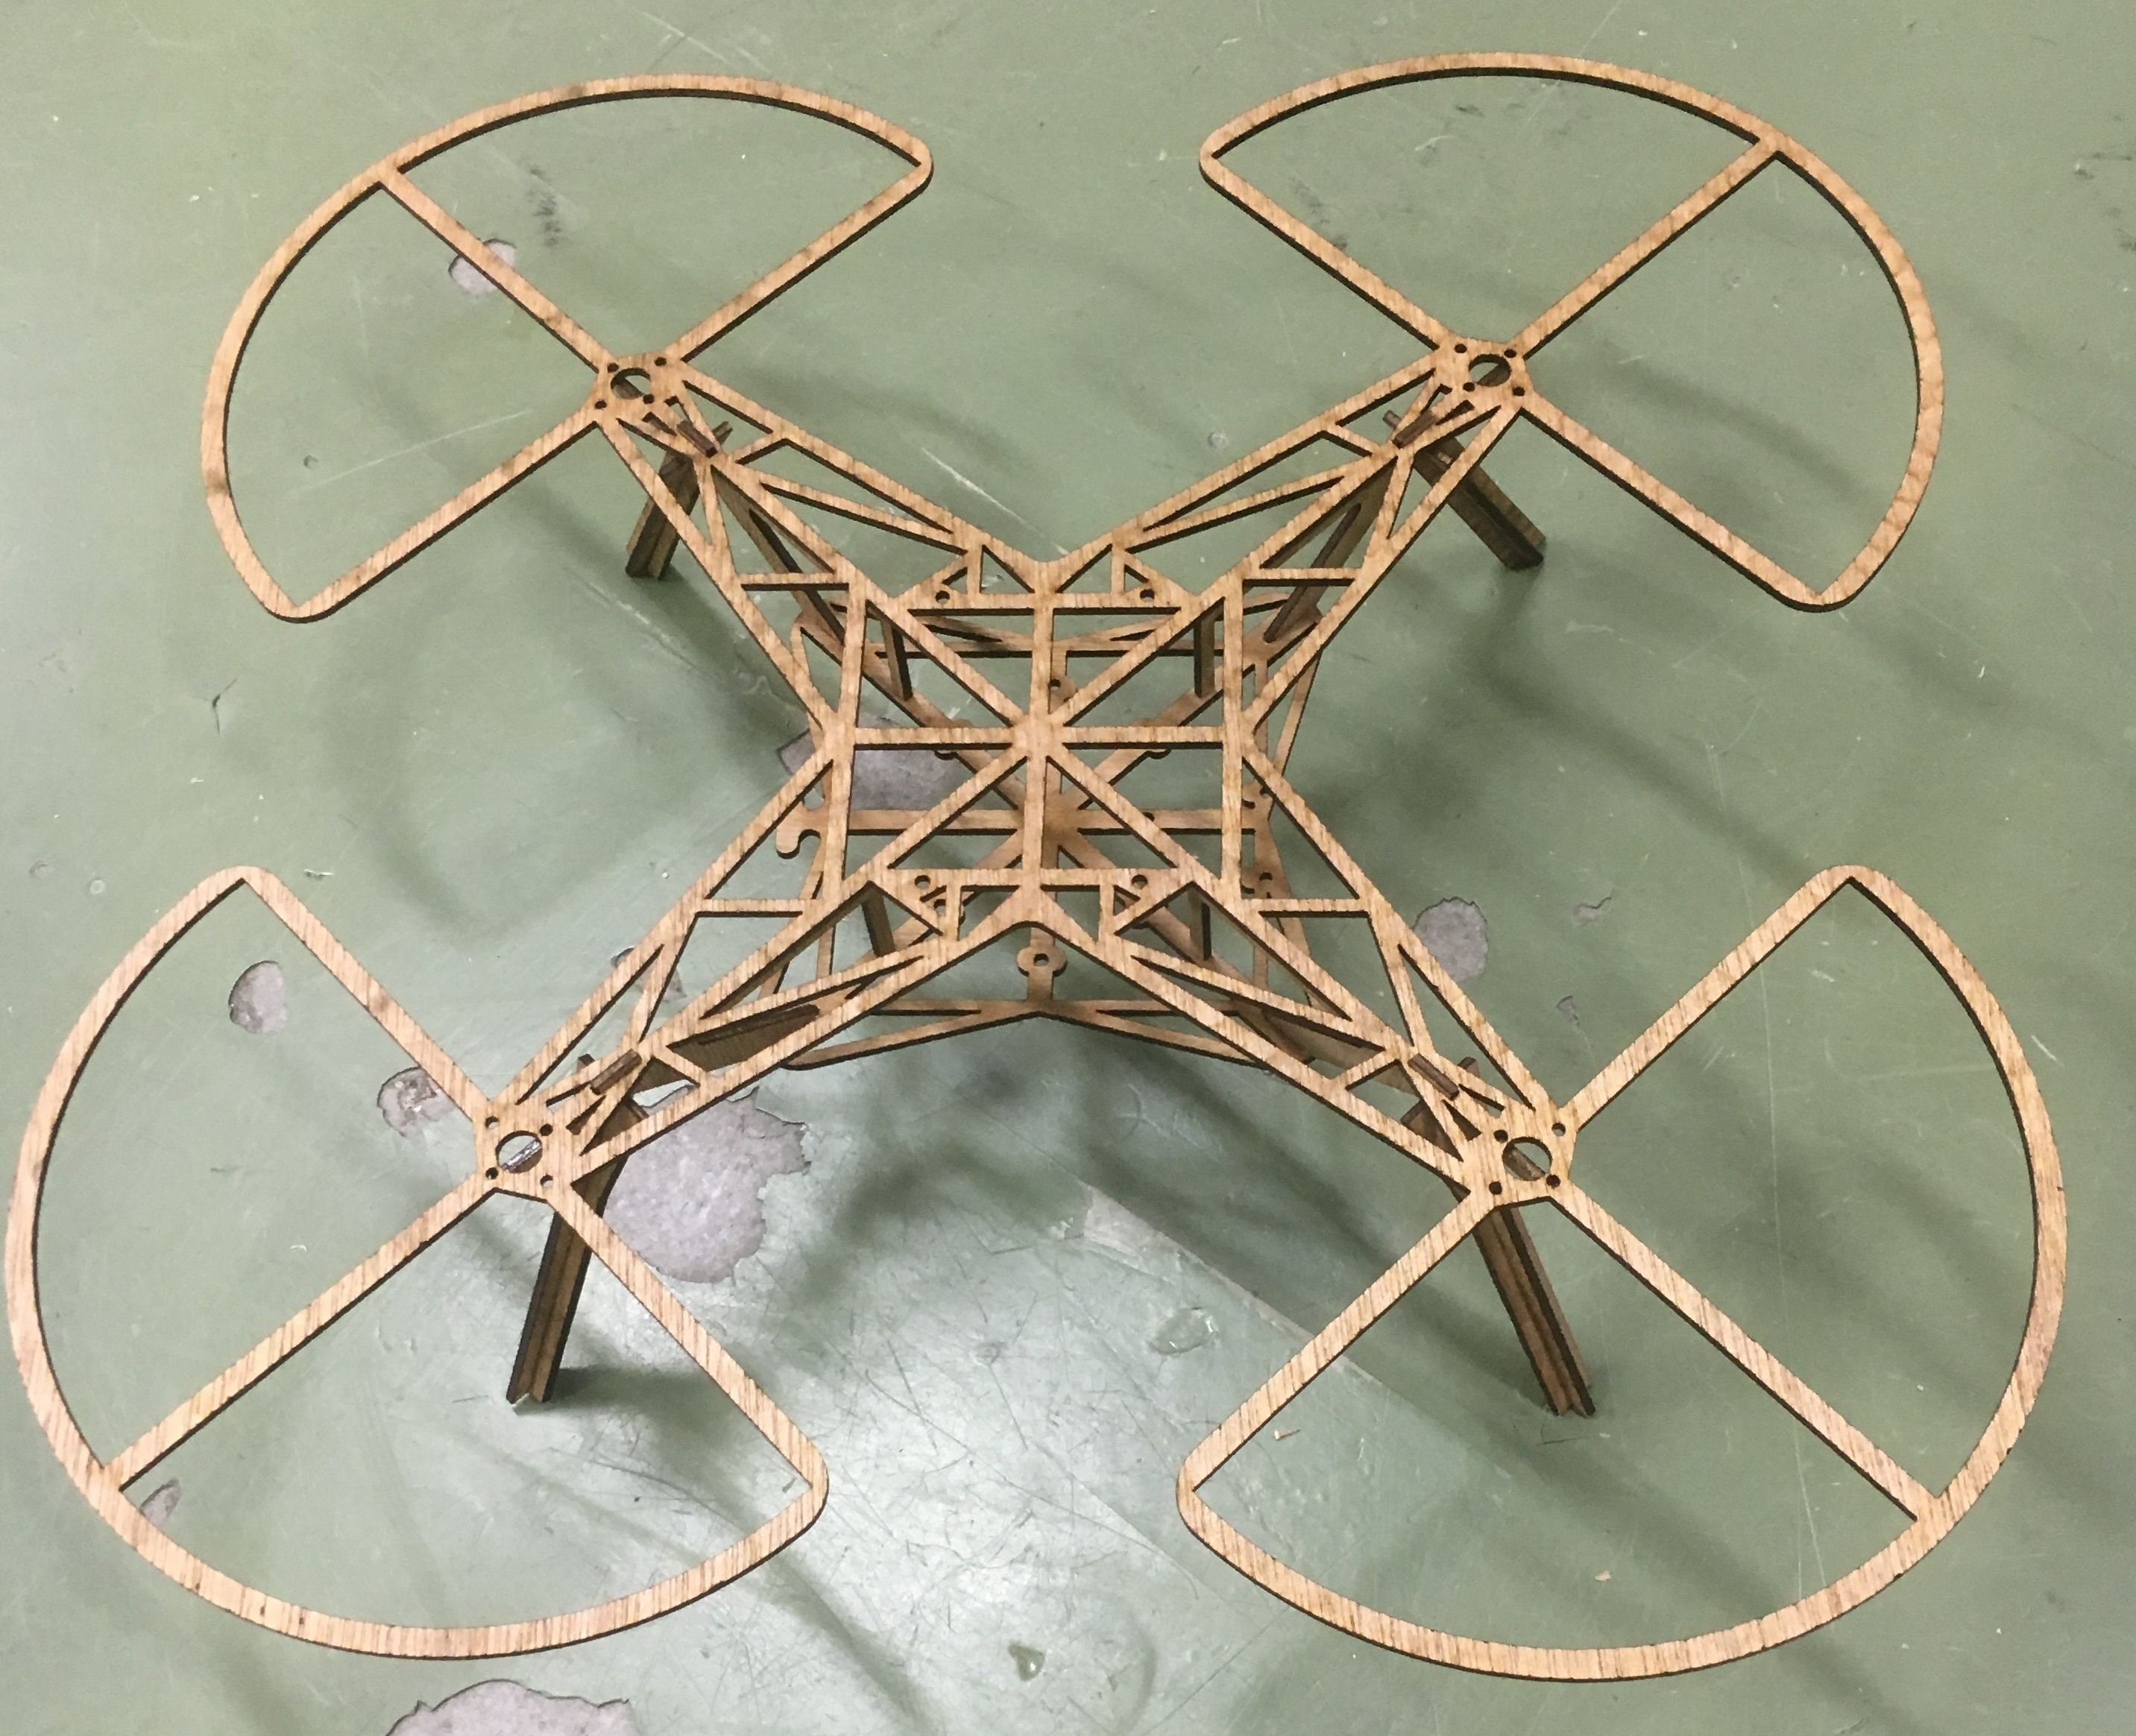
\includegraphics[width=100mm]{ga/thr.jpg}
    \end{center}
  \caption{改良その2}
 \label{fig:thr}
\end{figure}

ここでは主に形だけでは無く,使用するベニヤ板の密度が小さいものを使用した.その結果約40gほどまでに軽量化した.

\begin{figure}[H]
  \begin{center}
    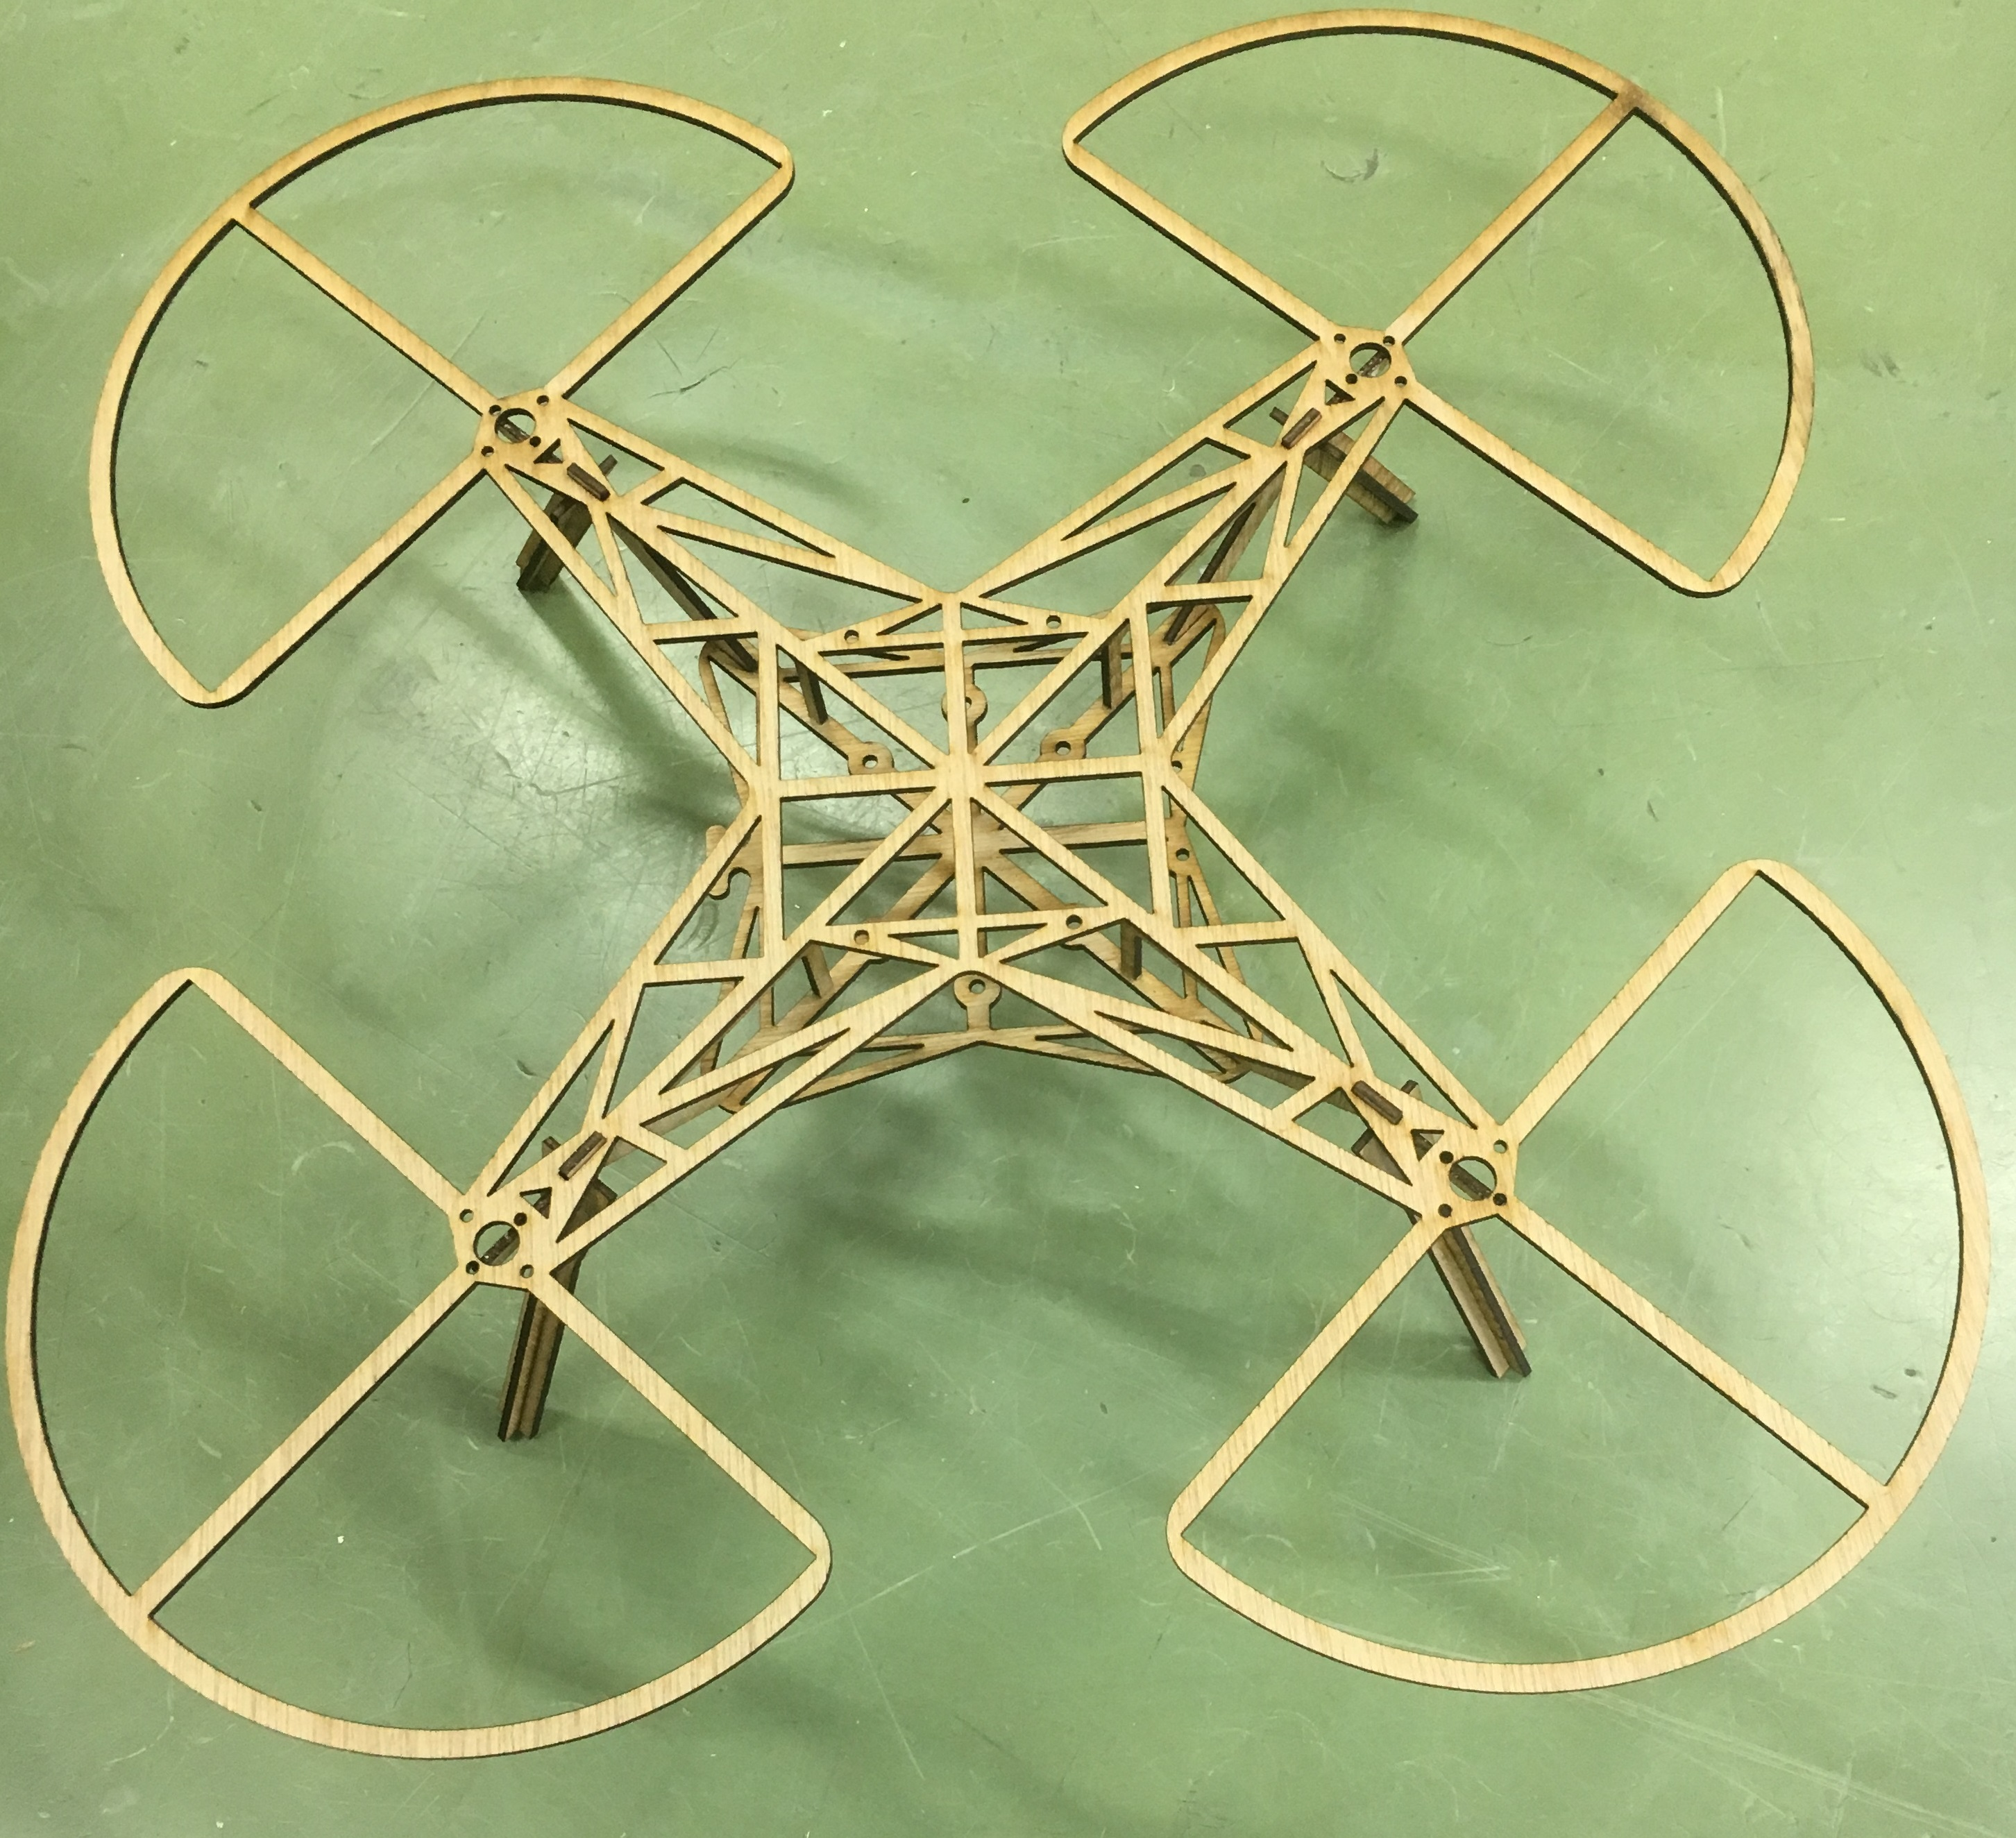
\includegraphics[width=100mm]{ga/fif.jpg}
    \end{center}
  \caption{改良その3}
 \label{fig:fif}
\end{figure}

\begin{figure}[H]
  \begin{center}
    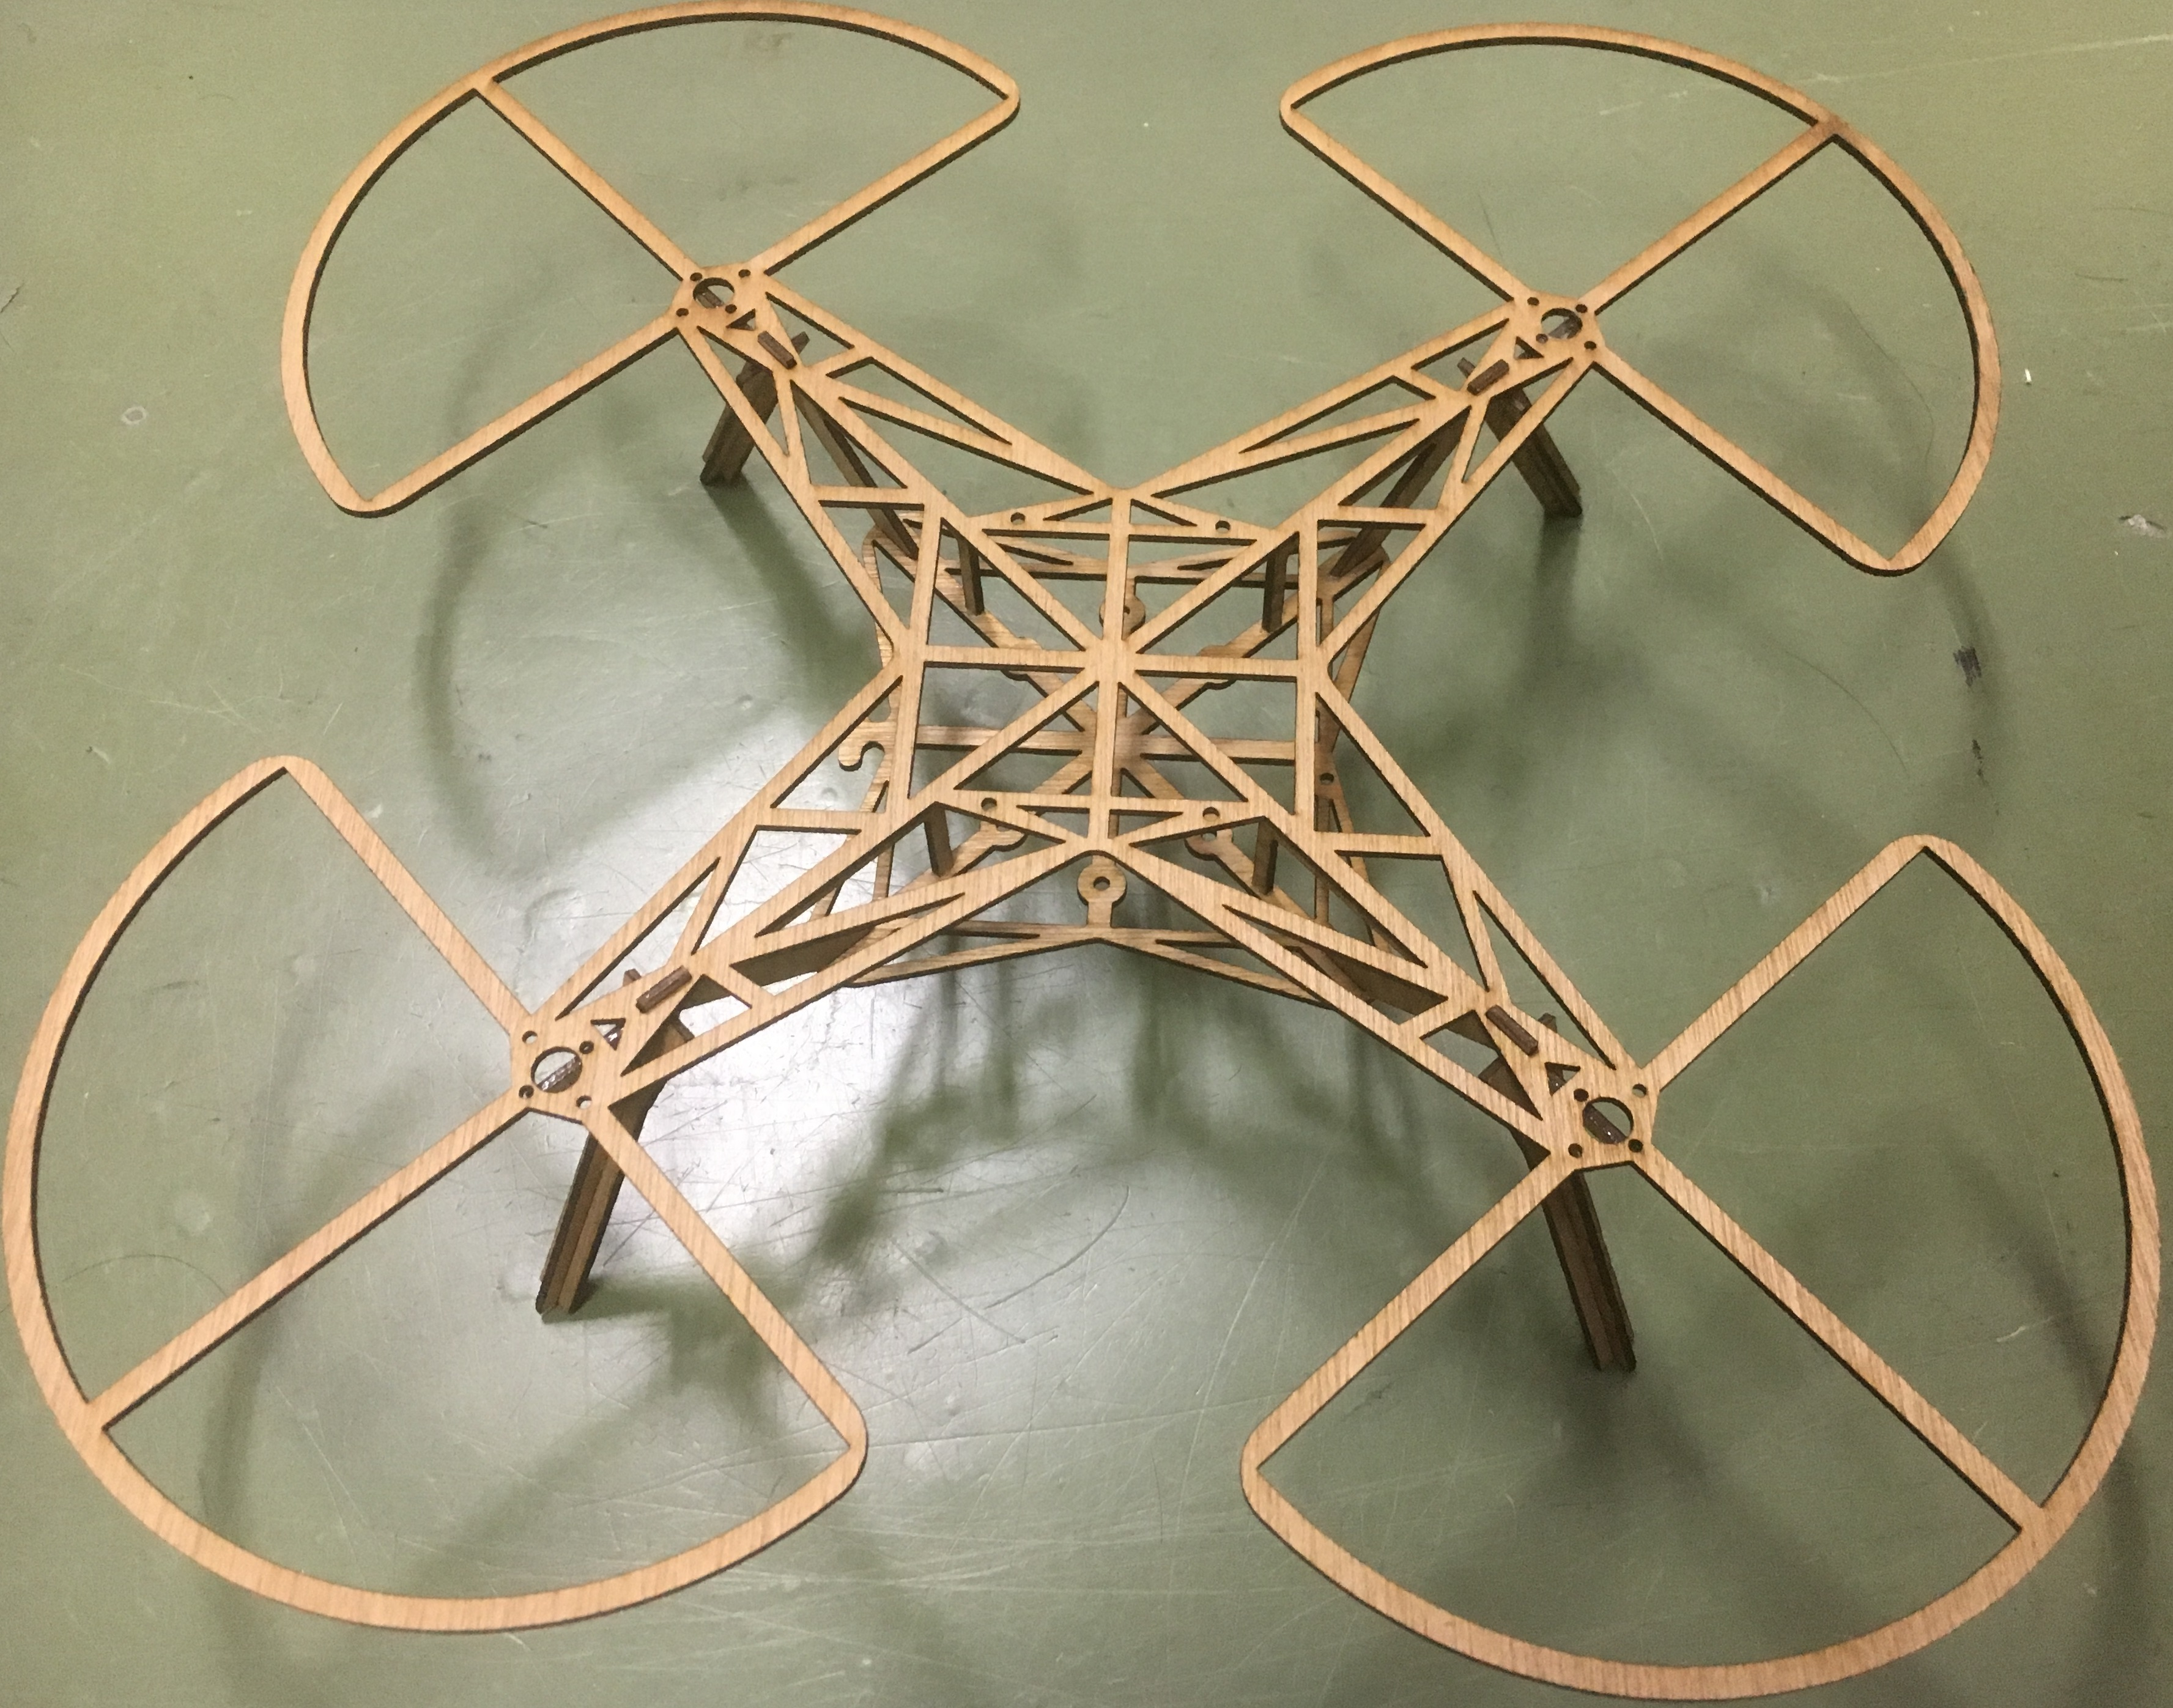
\includegraphics[width=100mm]{ga/flame.jpg}
    \end{center}
  \caption{完成したベニヤフレーム}
 \label{fig:flame}
\end{figure}

\section{製作}このフレーム形を手作業で製作するにはかなりの根気や技術,時間を必要とする.この製作を図\ref{fig:laser}のレーザー加工機を使用することによってこの形を綺麗に作るための技術や時間を短縮することに成功した.

\begin{figure}[H]
  \begin{center}
    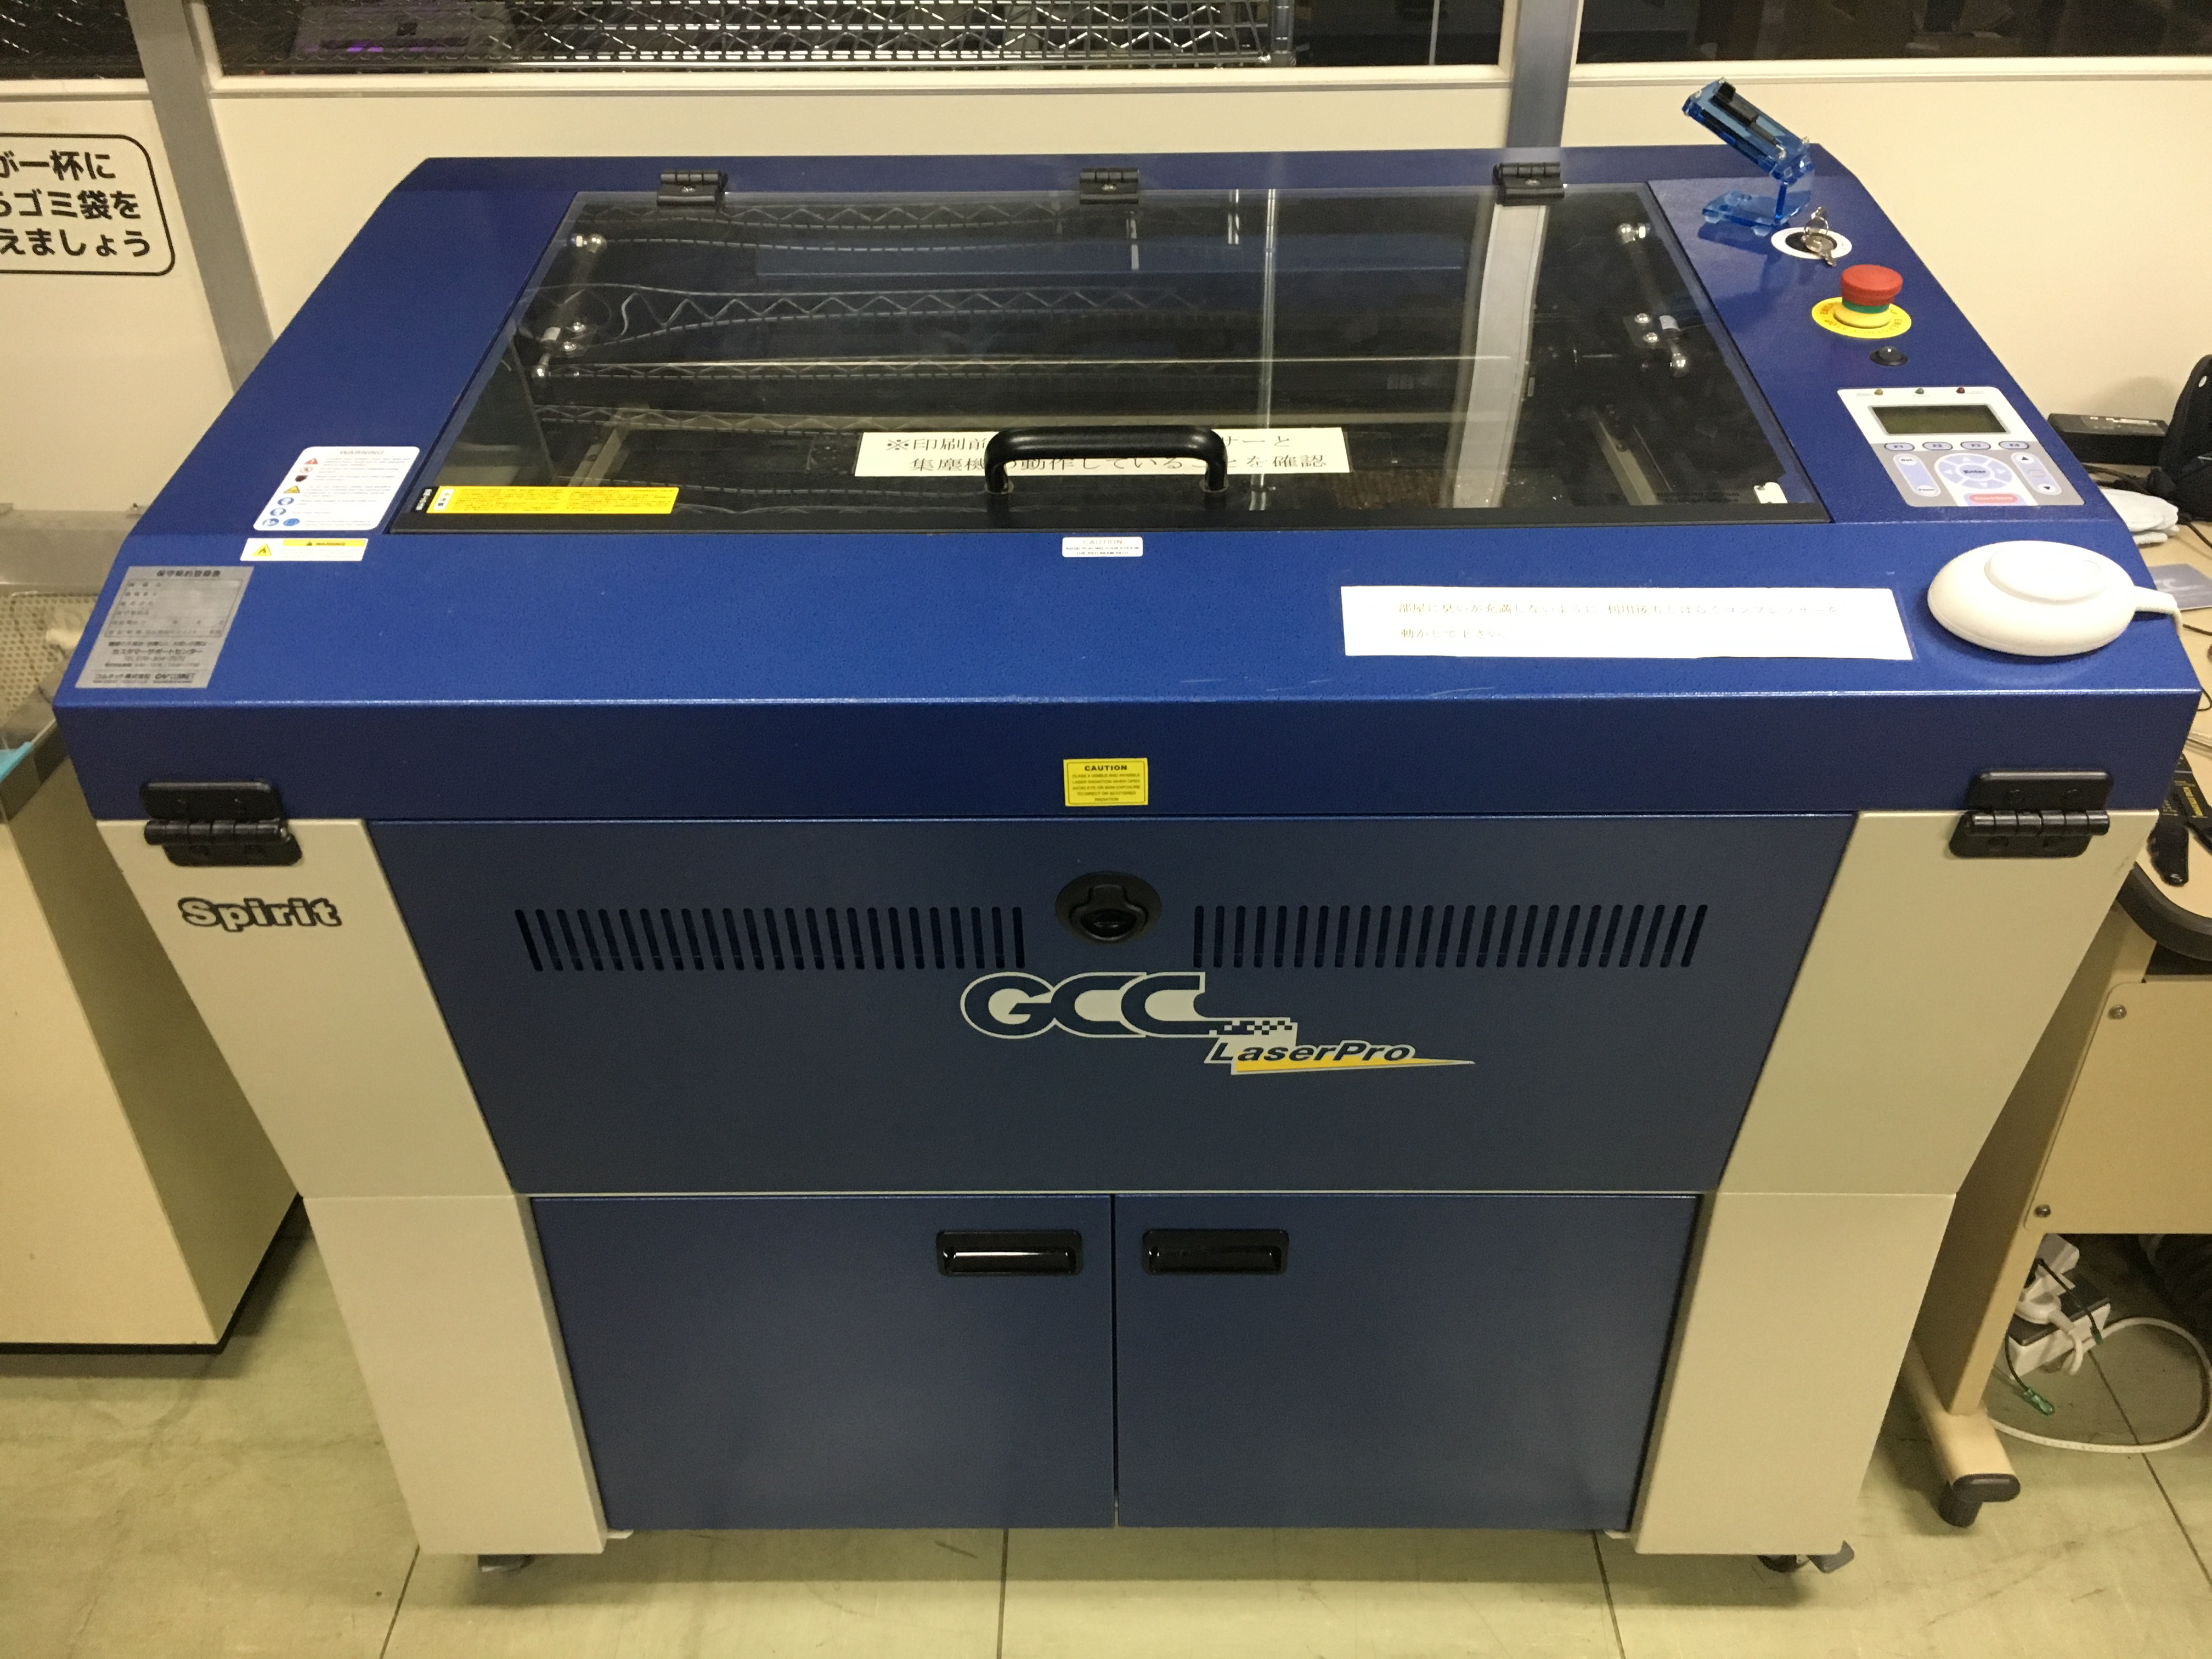
\includegraphics[width=100mm]{ga/laser.jpeg}
    \end{center}
  \caption{レーザー加工機}
 \label{fig:laser}
\end{figure}

\chapter{回路設計製作}
\section{ドローンの制御システム}今回自作する制御システムのブロック線図を図\ref{fig:brok}に記す.

\begin{figure}[H]
  \begin{center}
    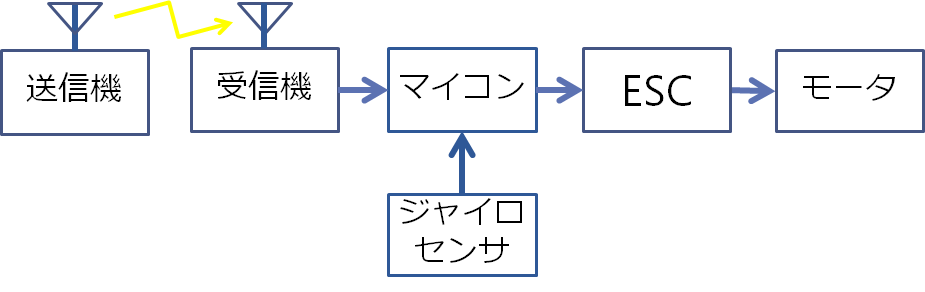
\includegraphics[width=110mm]{ga/brok.png}
    \end{center}
  \caption{制御システムブロック線図}
 \label{fig:brok}
\end{figure}

この流れは送信機からの指示を受信機で受け取りマイコン内でセンサーからのデータとともに処理することで出力するデータを出す.
その後,ESCに送りその信号でモーターを回転させる.
このESCとはマイコンからの信号によりモーターの回転速度を制御するモータードライバーの一種である.


\section{使用する電子部品}
今回の製作に必要な電子部品は以下のようとなる.

\begin{enumerate}
\item マイコン
\item ジャイロ
\item ESC
\item モータ
\item 受信機
\item 送信機
\item バッテリー
\item 電源関係
\end{enumerate}

このドローンの頭脳ともいえるセンサーや図\ref{fig:R2006GS}の受信機からのデータを処理しESCにモーターの回転数を指示する信号を送ったりするマイコンは図にある秋月電子のRX621で,センサーは図\ref{fig:RX621}の秋月電子のRX621を使用する.

\begin{figure}[H]
\begin{center}
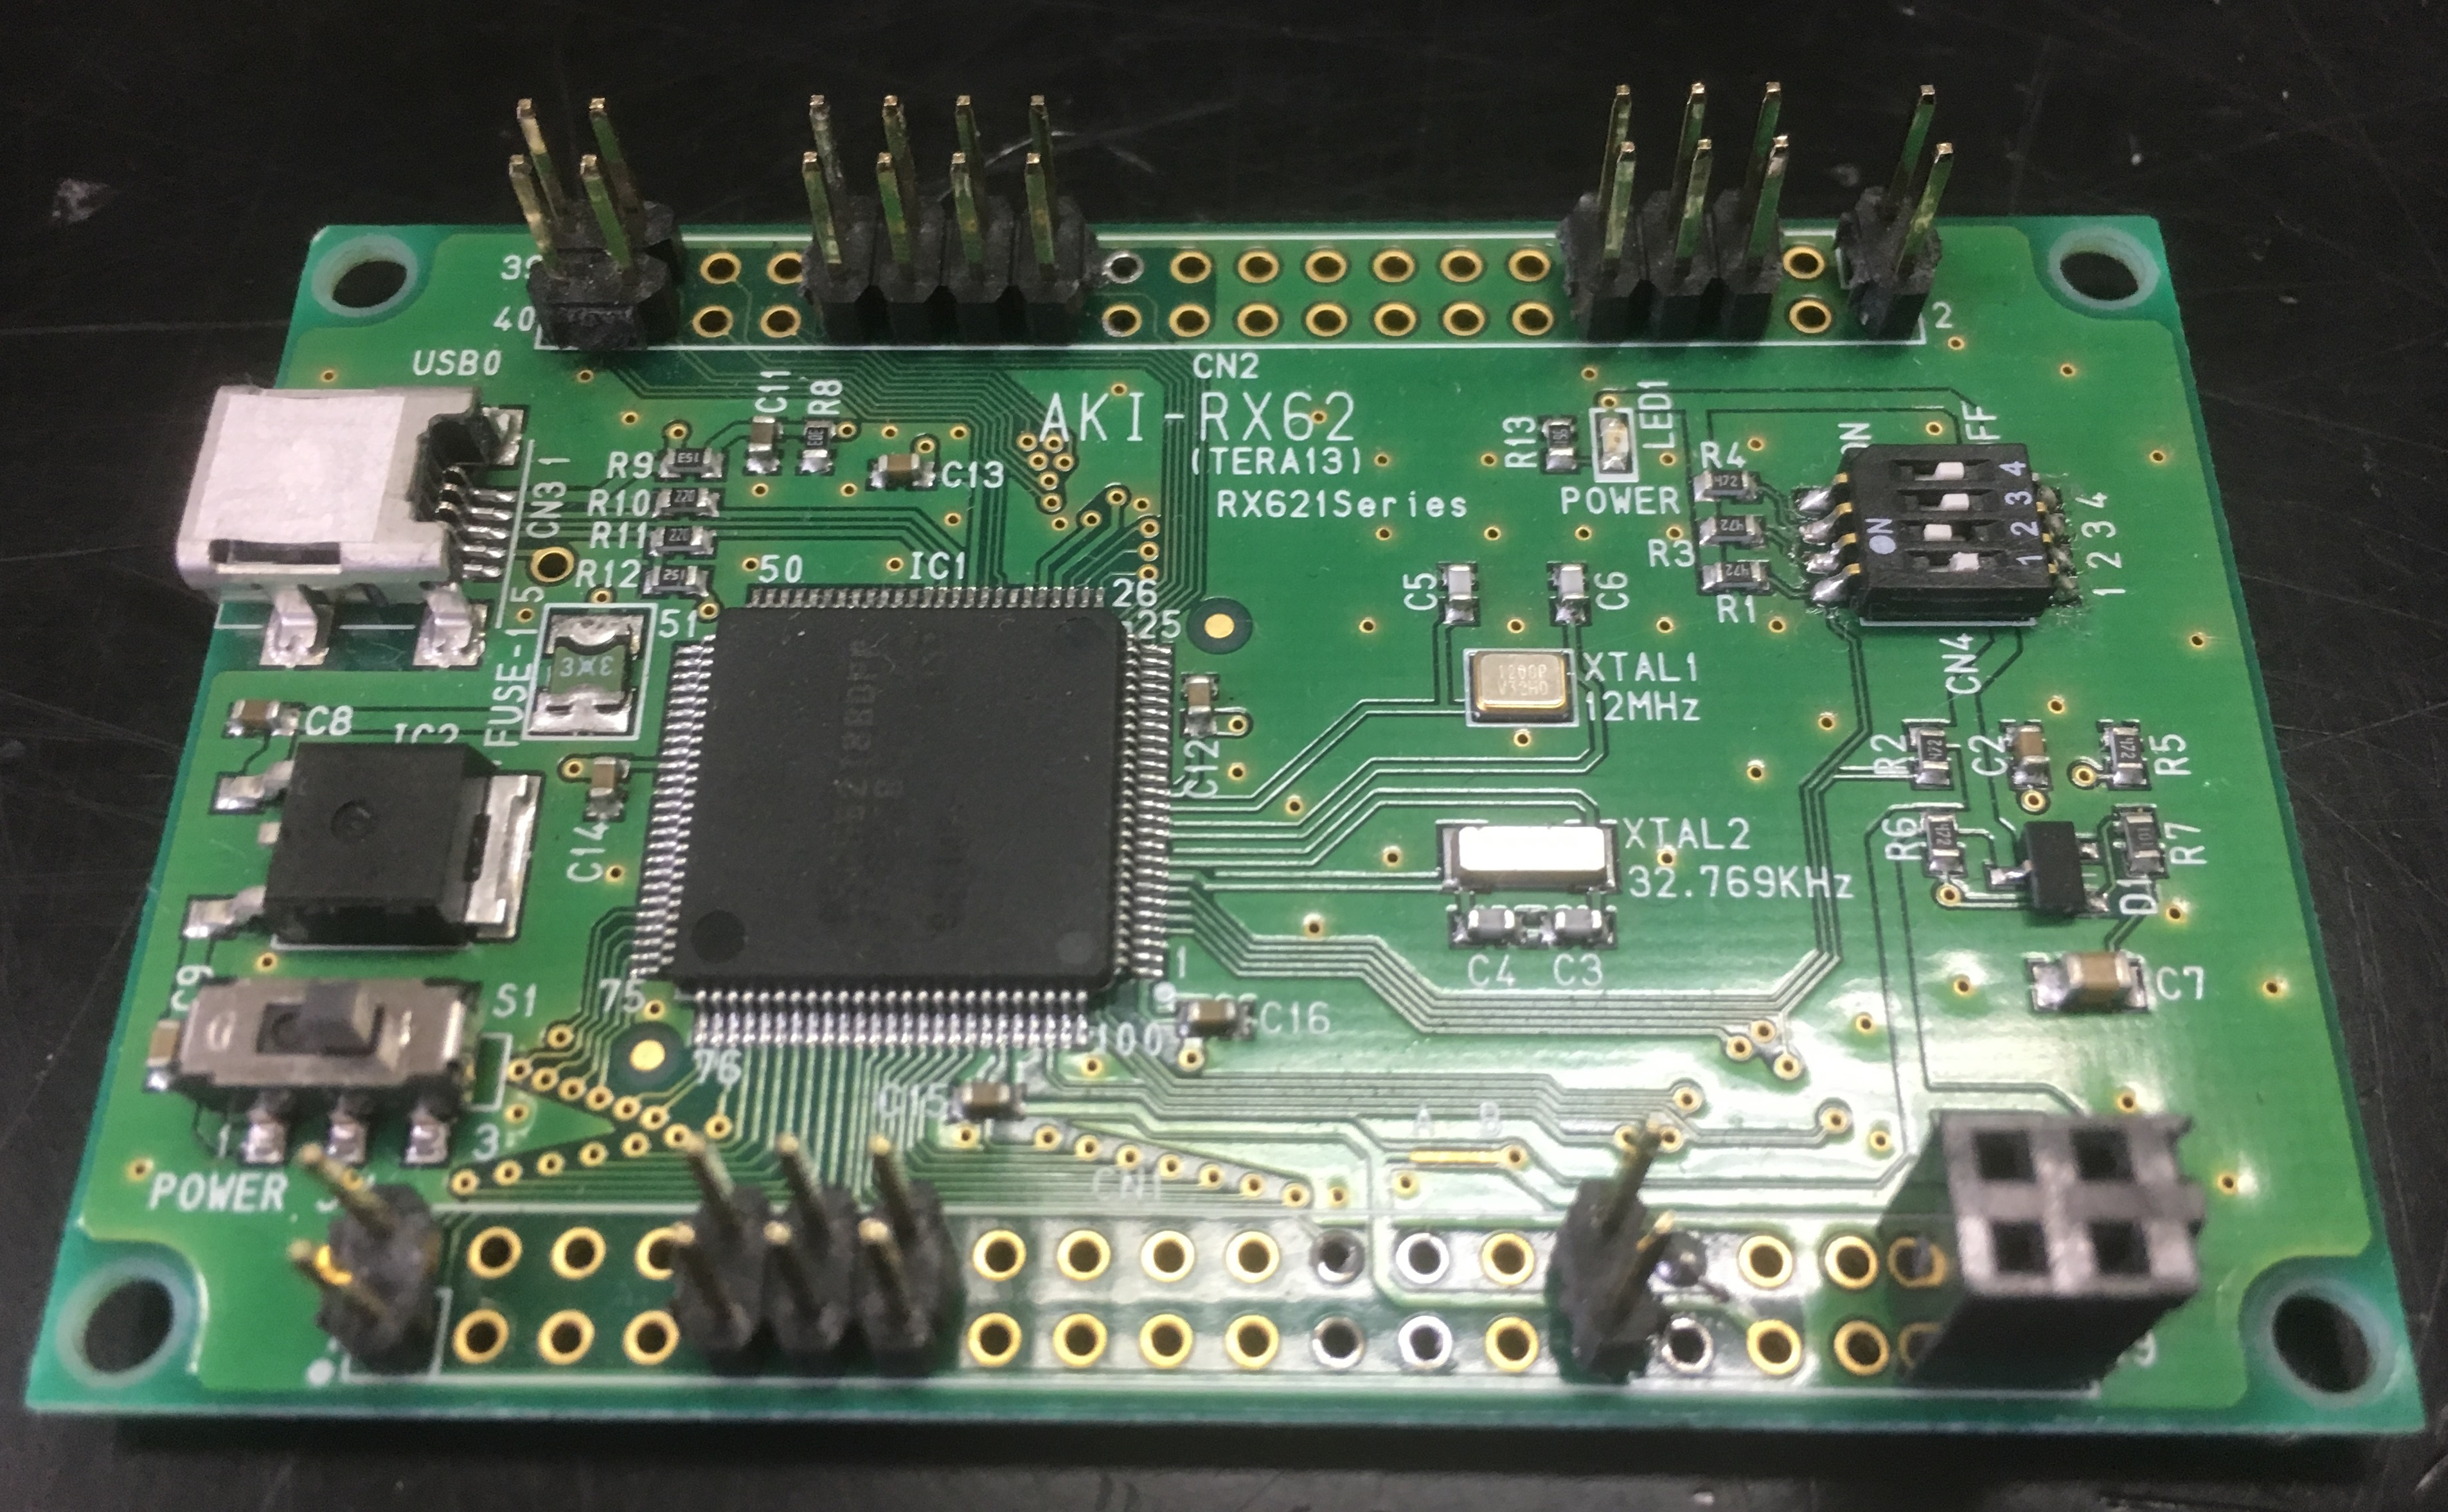
\includegraphics[width=90mm]{ga/RX621.jpg}
\end{center}
\caption{マイコン}
\label{fig:RX621}
\end{figure}

\begin{figure}[H]
\begin{center}
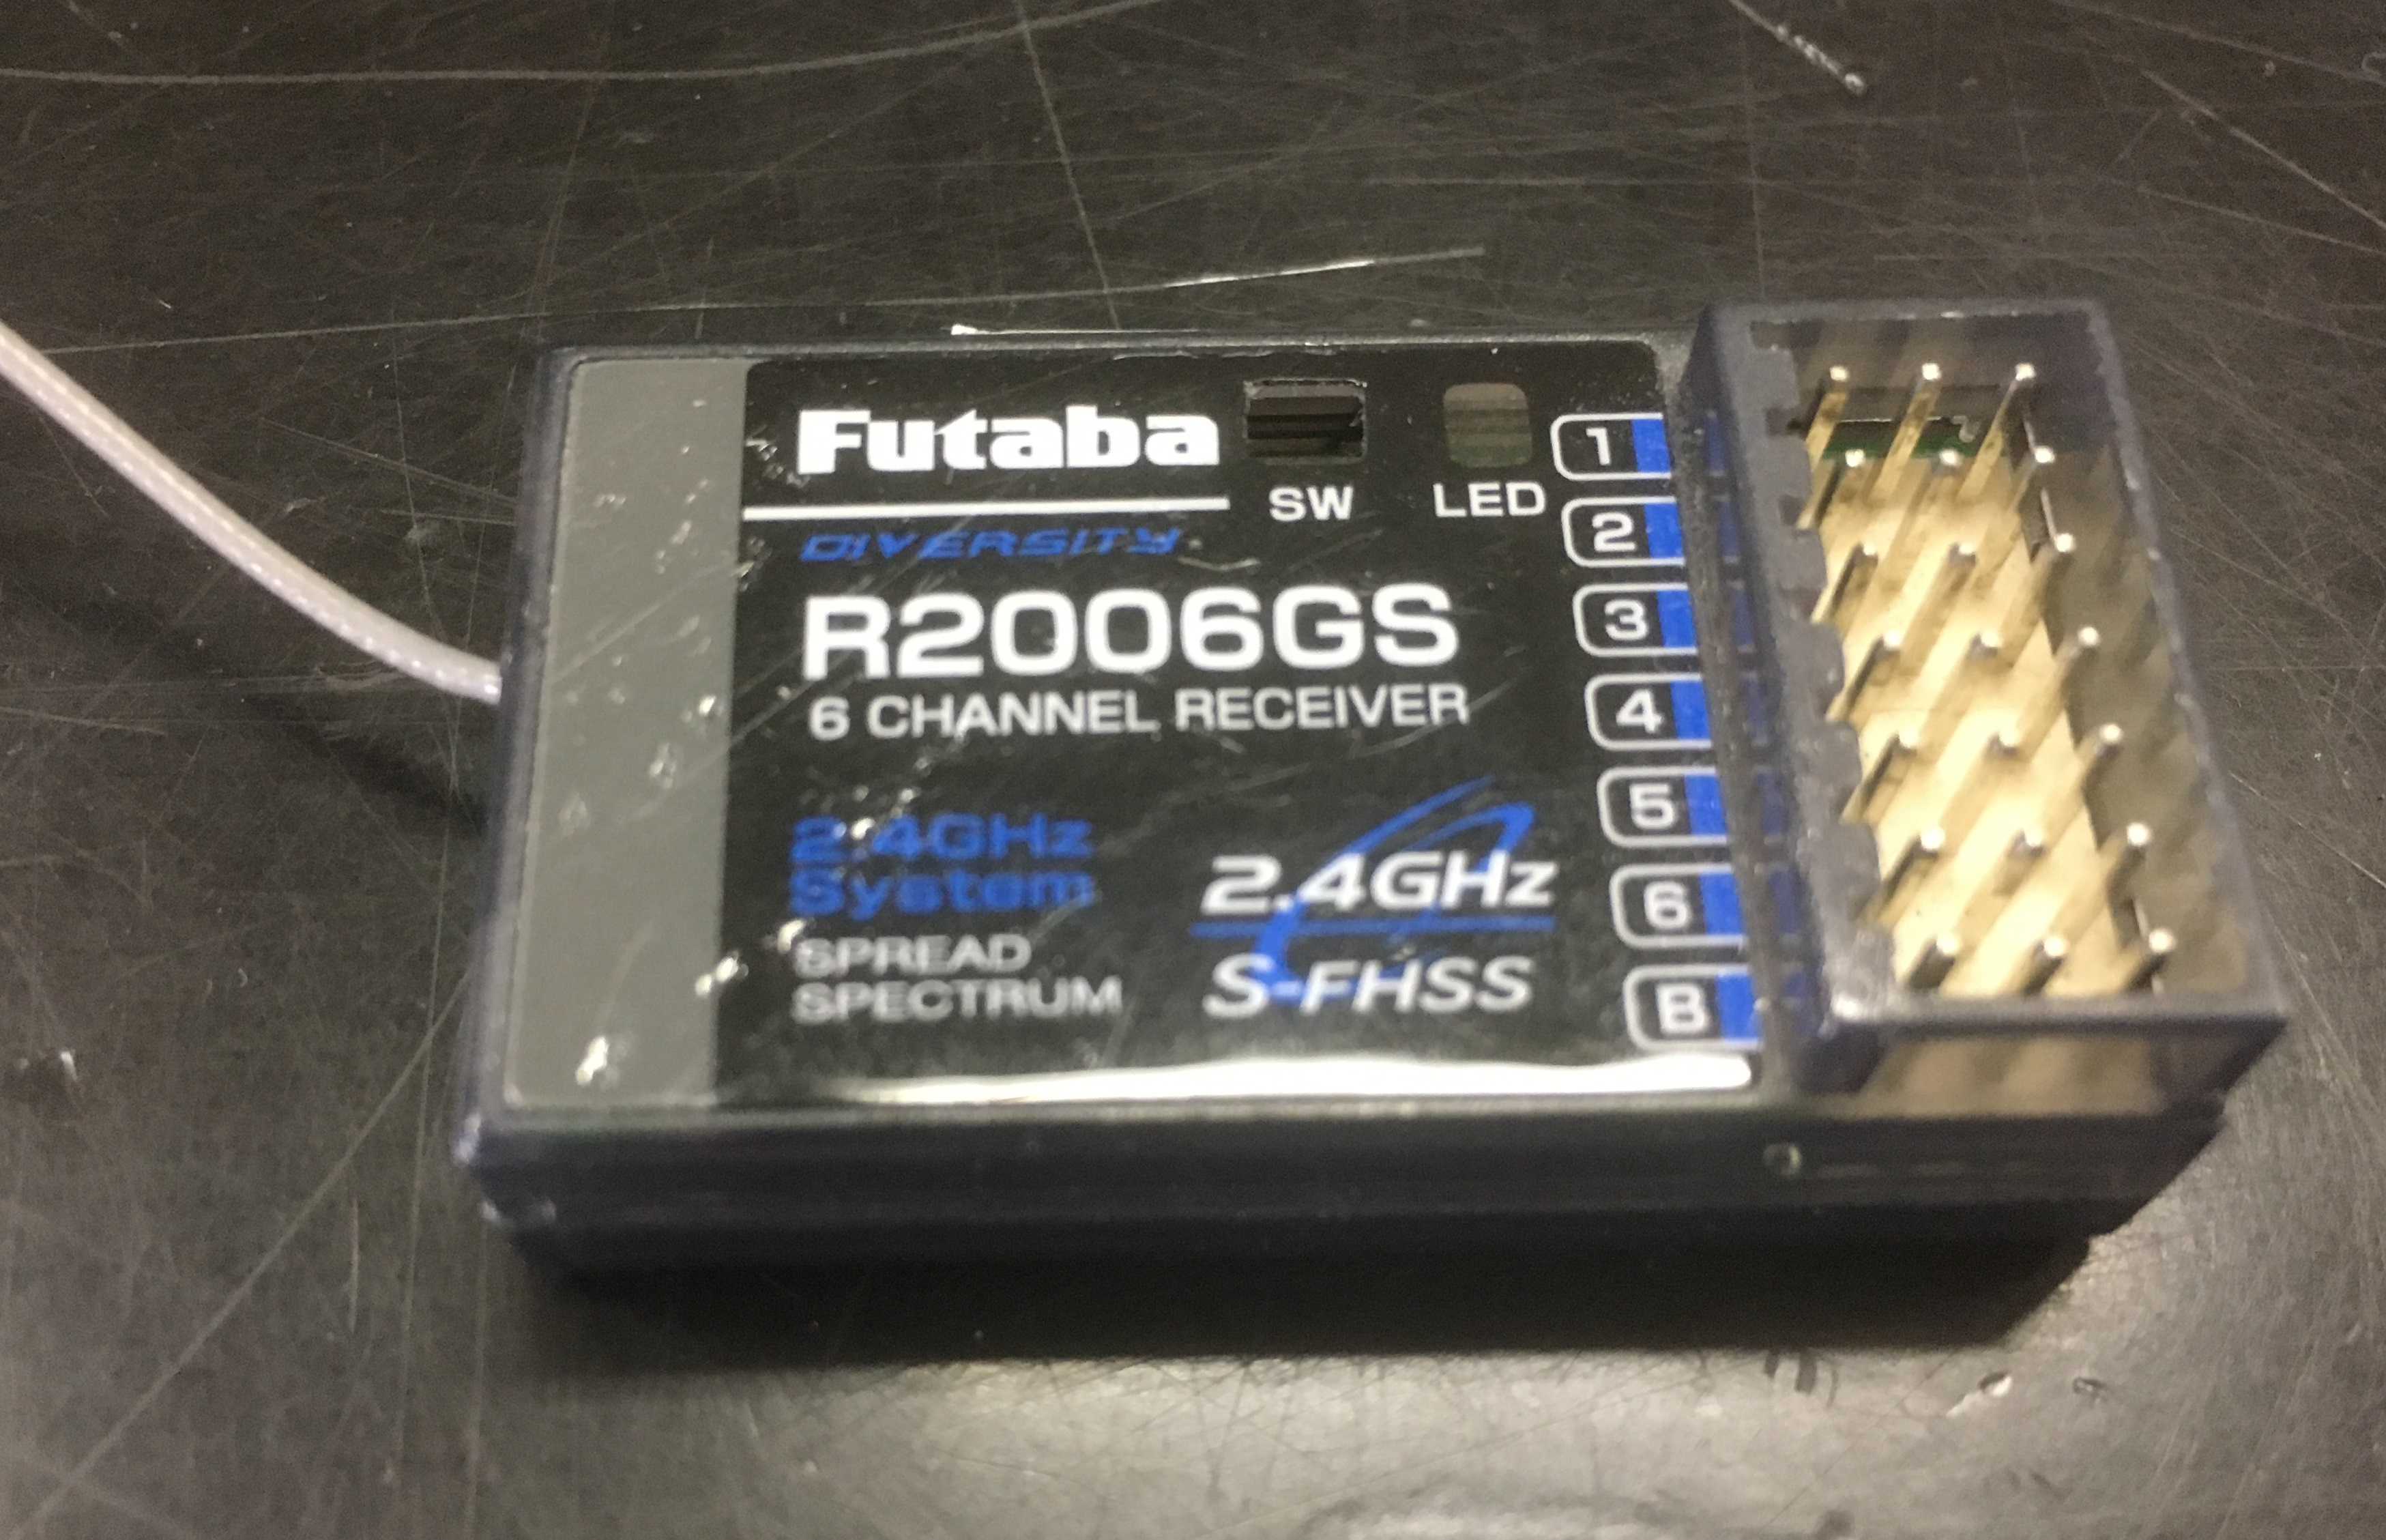
\includegraphics[width=90mm]{ga/res.jpg}
\end{center}
\caption{受信機}
\label{fig:R2006GS}
\end{figure}

今回の研究の要となるセンサーは図\ref{fig:GY-80}のGY-80というジャイロ,加速度,地磁気といった複数のセンサーが一つとなったもので,その中のジャイロセンサだけを使用する.

\begin{figure}[H]
\begin{center}
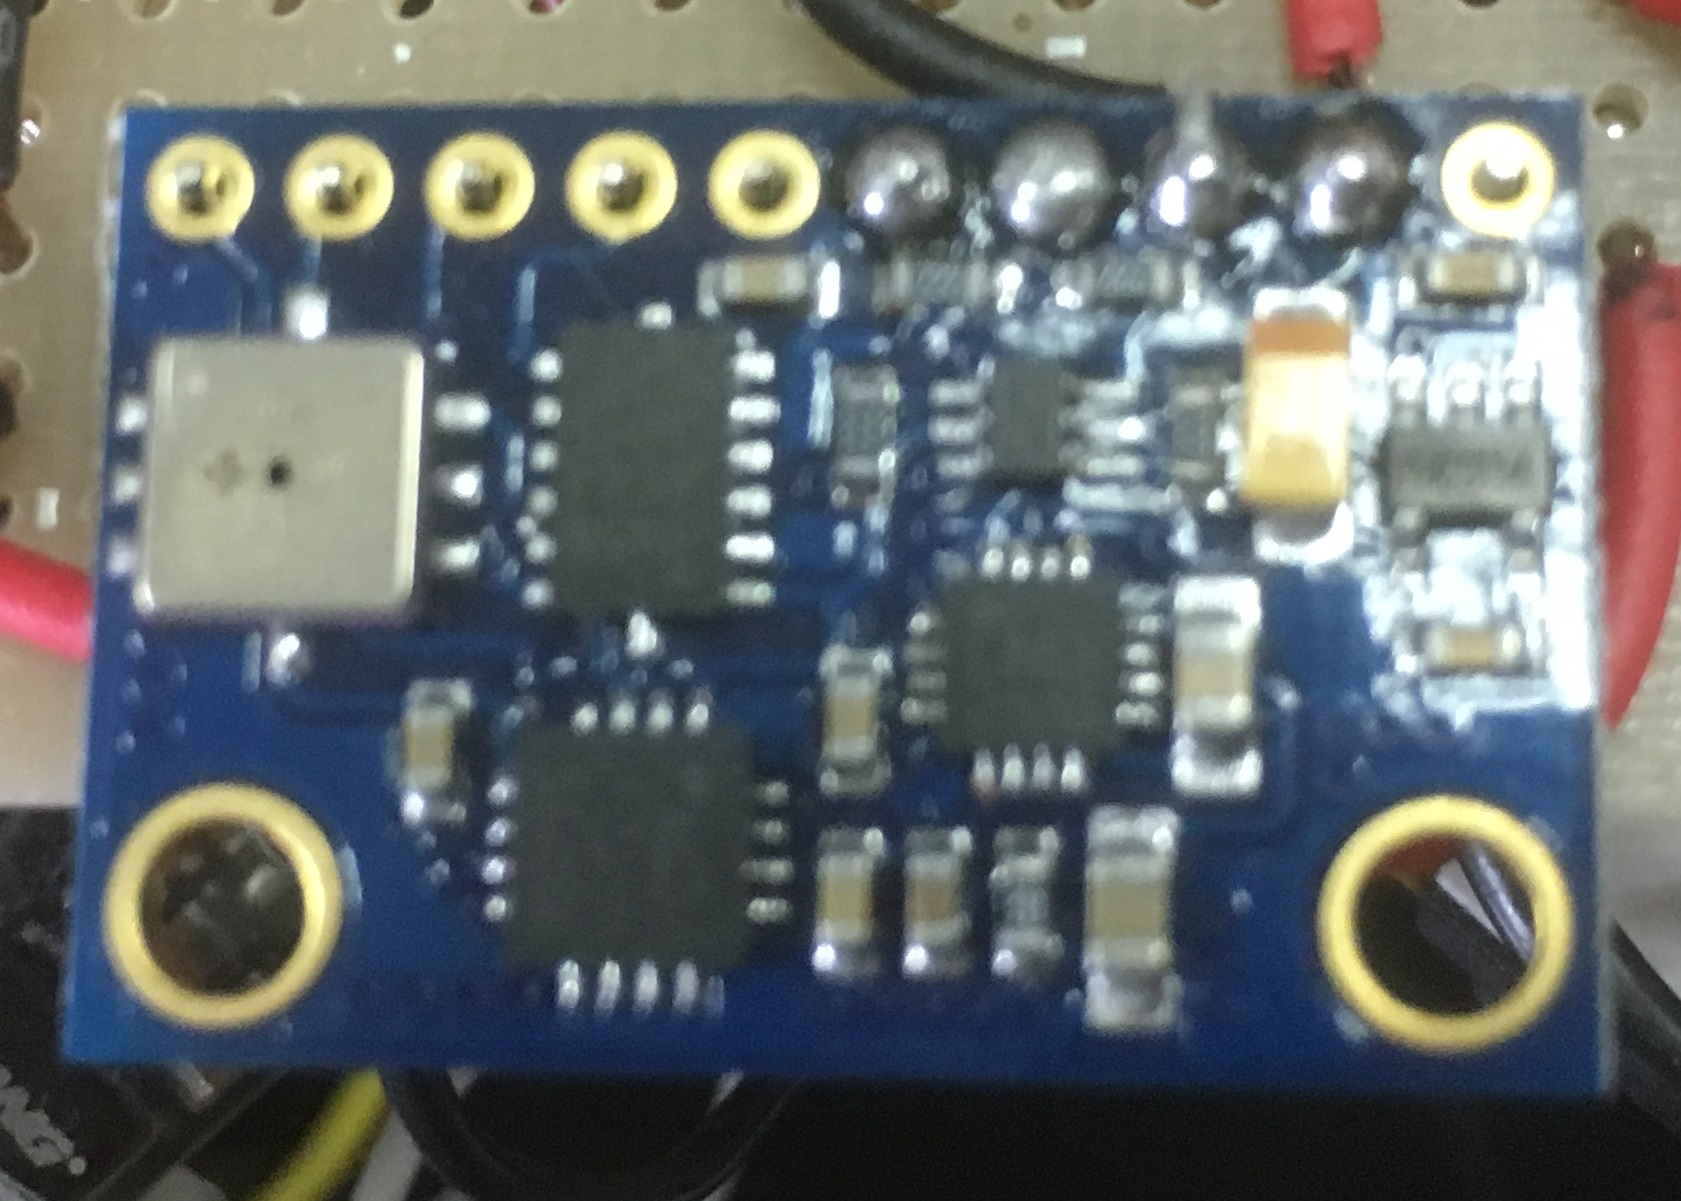
\includegraphics[width=90mm]{ga/GY-80.jpg}
\end{center}
\caption{ジャイロセンサー}
\label{fig:GY-80}
\end{figure}

ドローンを飛ばすためのモーターは図\ref{fig:MN1804-KV2400},マイコンからの指示をモーターへと繋ぐためのESCは図\ref{fig:30A Micro 2-4S}を使用する.

\begin{figure}[H]
\begin{center}
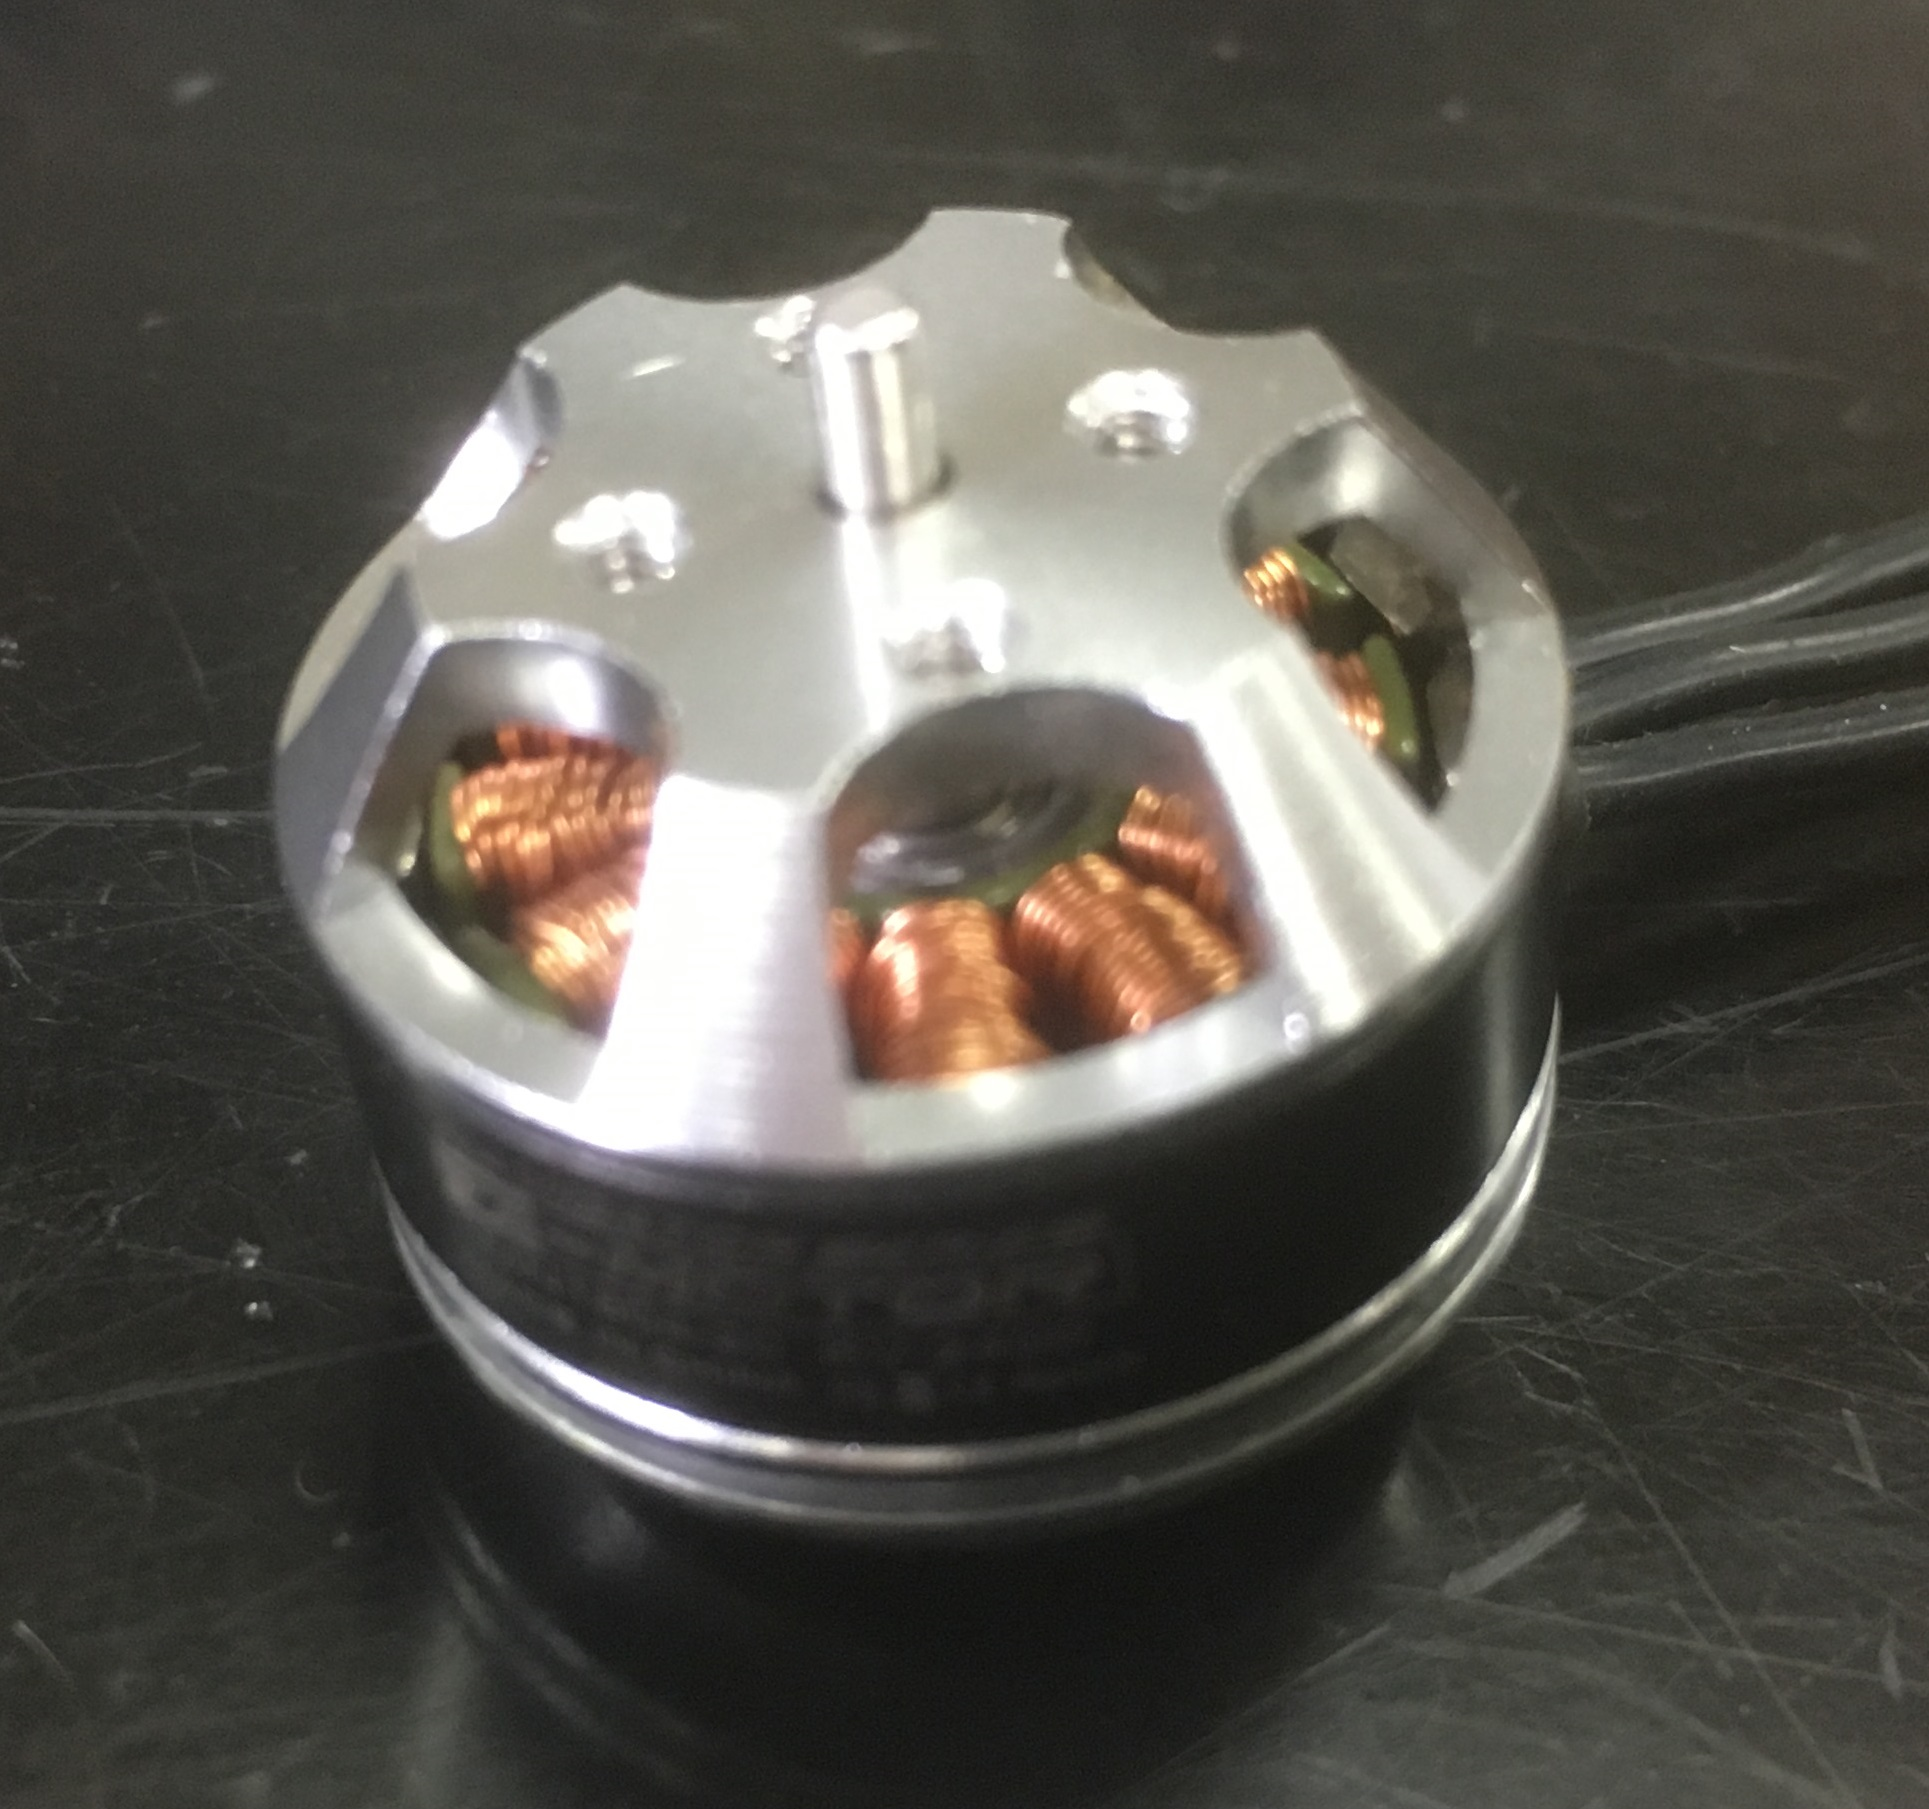
\includegraphics[width=90mm]{ga/mot.jpg}
\end{center}
\caption{モーター}
\label{fig:MN1804-KV2400}
\end{figure}

\begin{figure}[H]
\begin{center}
\includegraphics[width=90mm]{ga/esc.jpg}
\end{center}
\caption{ESC}
\label{fig:30A Micro 2-4S}
\end{figure}

図\ref{fig:T850/35-2S}のバッテリーはドローンの電源で7.4Vの電圧を持っている.しかしマイコンとセンサーは3.3V,受信機は5Vの電圧を必要としているため図\ref{fig:P5293-33}のレギュレータで3.3V,図\ref{fig:MCW103-12S05}のDCDCコンバータで5Vに電圧を変換して使用する.

\begin{figure}[H]
\begin{center}
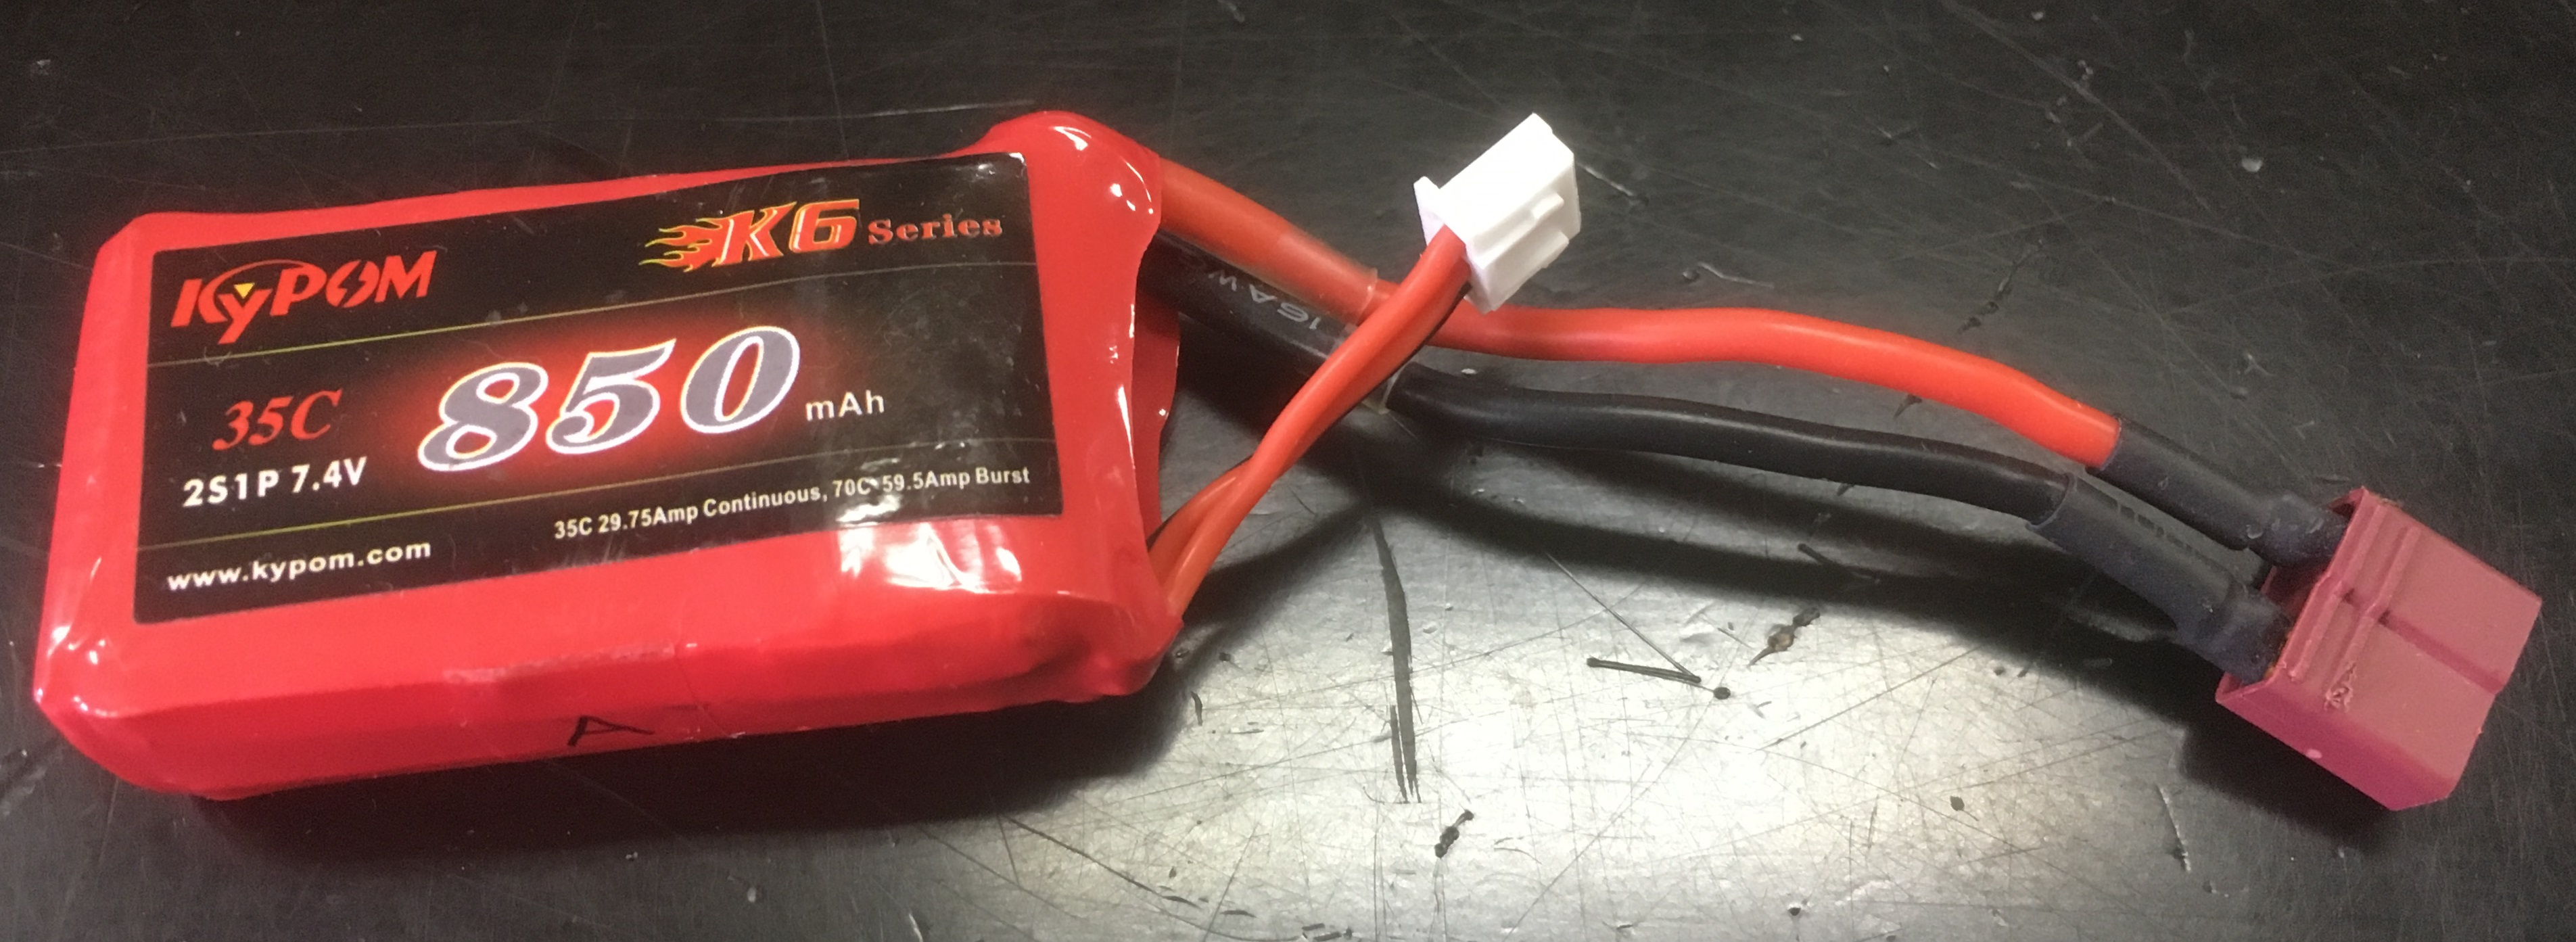
\includegraphics[width=90mm]{ga/bat.jpg}
\end{center}
\caption{バッテリー}
\label{fig:T850/35-2S}
\end{figure}

\begin{figure}[H]
\begin{center}
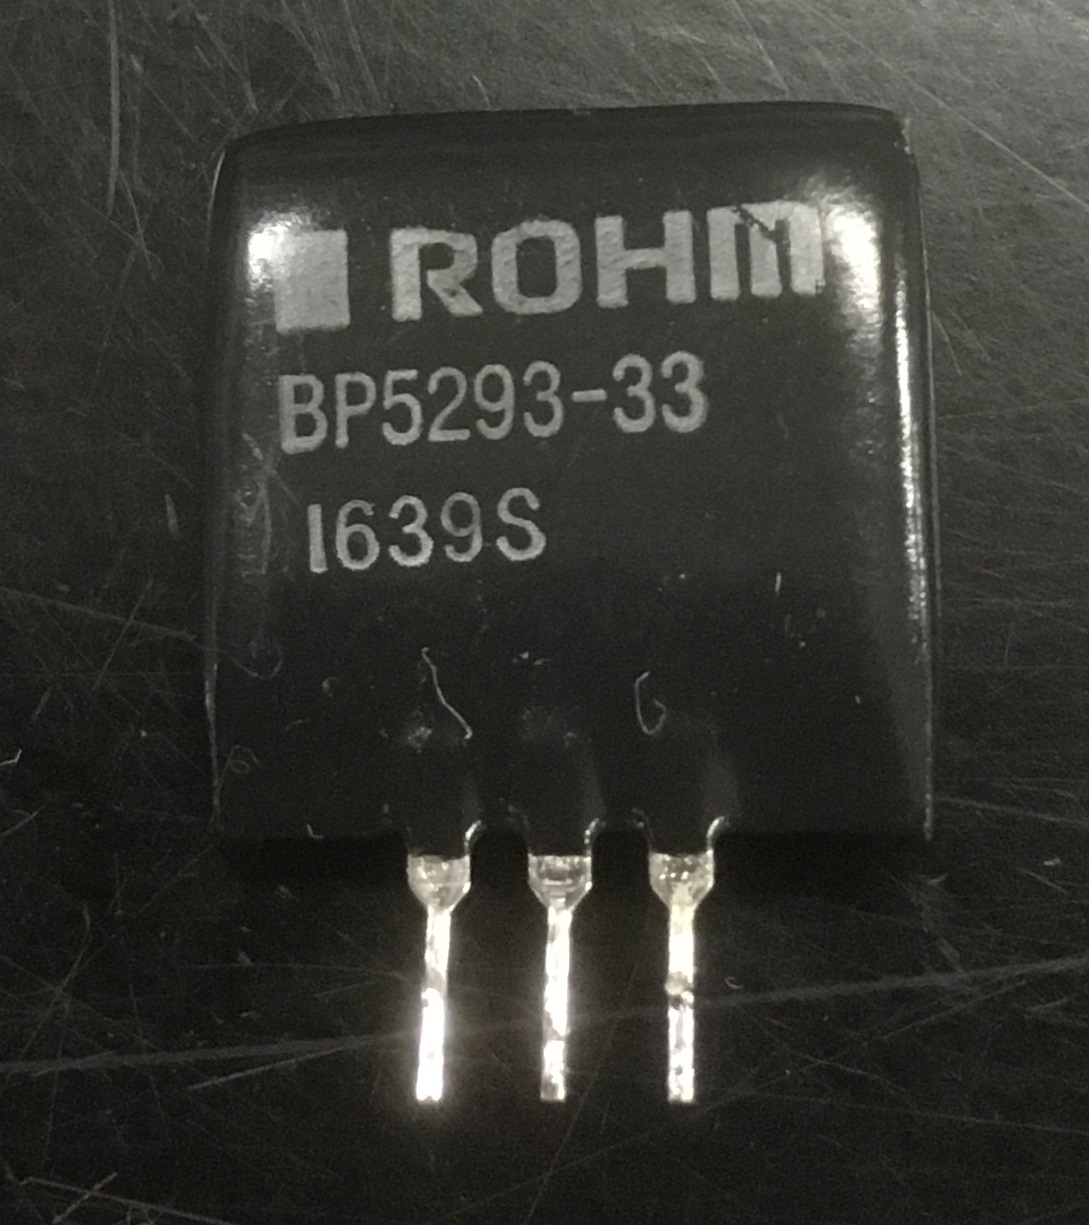
\includegraphics[width=90mm]{ga/reg.jpg}
\end{center}
\caption{レギュレータ}
\label{fig:P5293-33}
\end{figure}

\begin{figure}[H]
\begin{center}
\includegraphics[width=90mm]{ga/dcdc.jpg}
\end{center}
\caption{DCDCコンバータ}
\label{fig:MCW103-12S05}
\end{figure}

以上の部品を使用し製作した基板が図\ref{fig:kairo}となる.

\begin{figure}[H]
\begin{center}
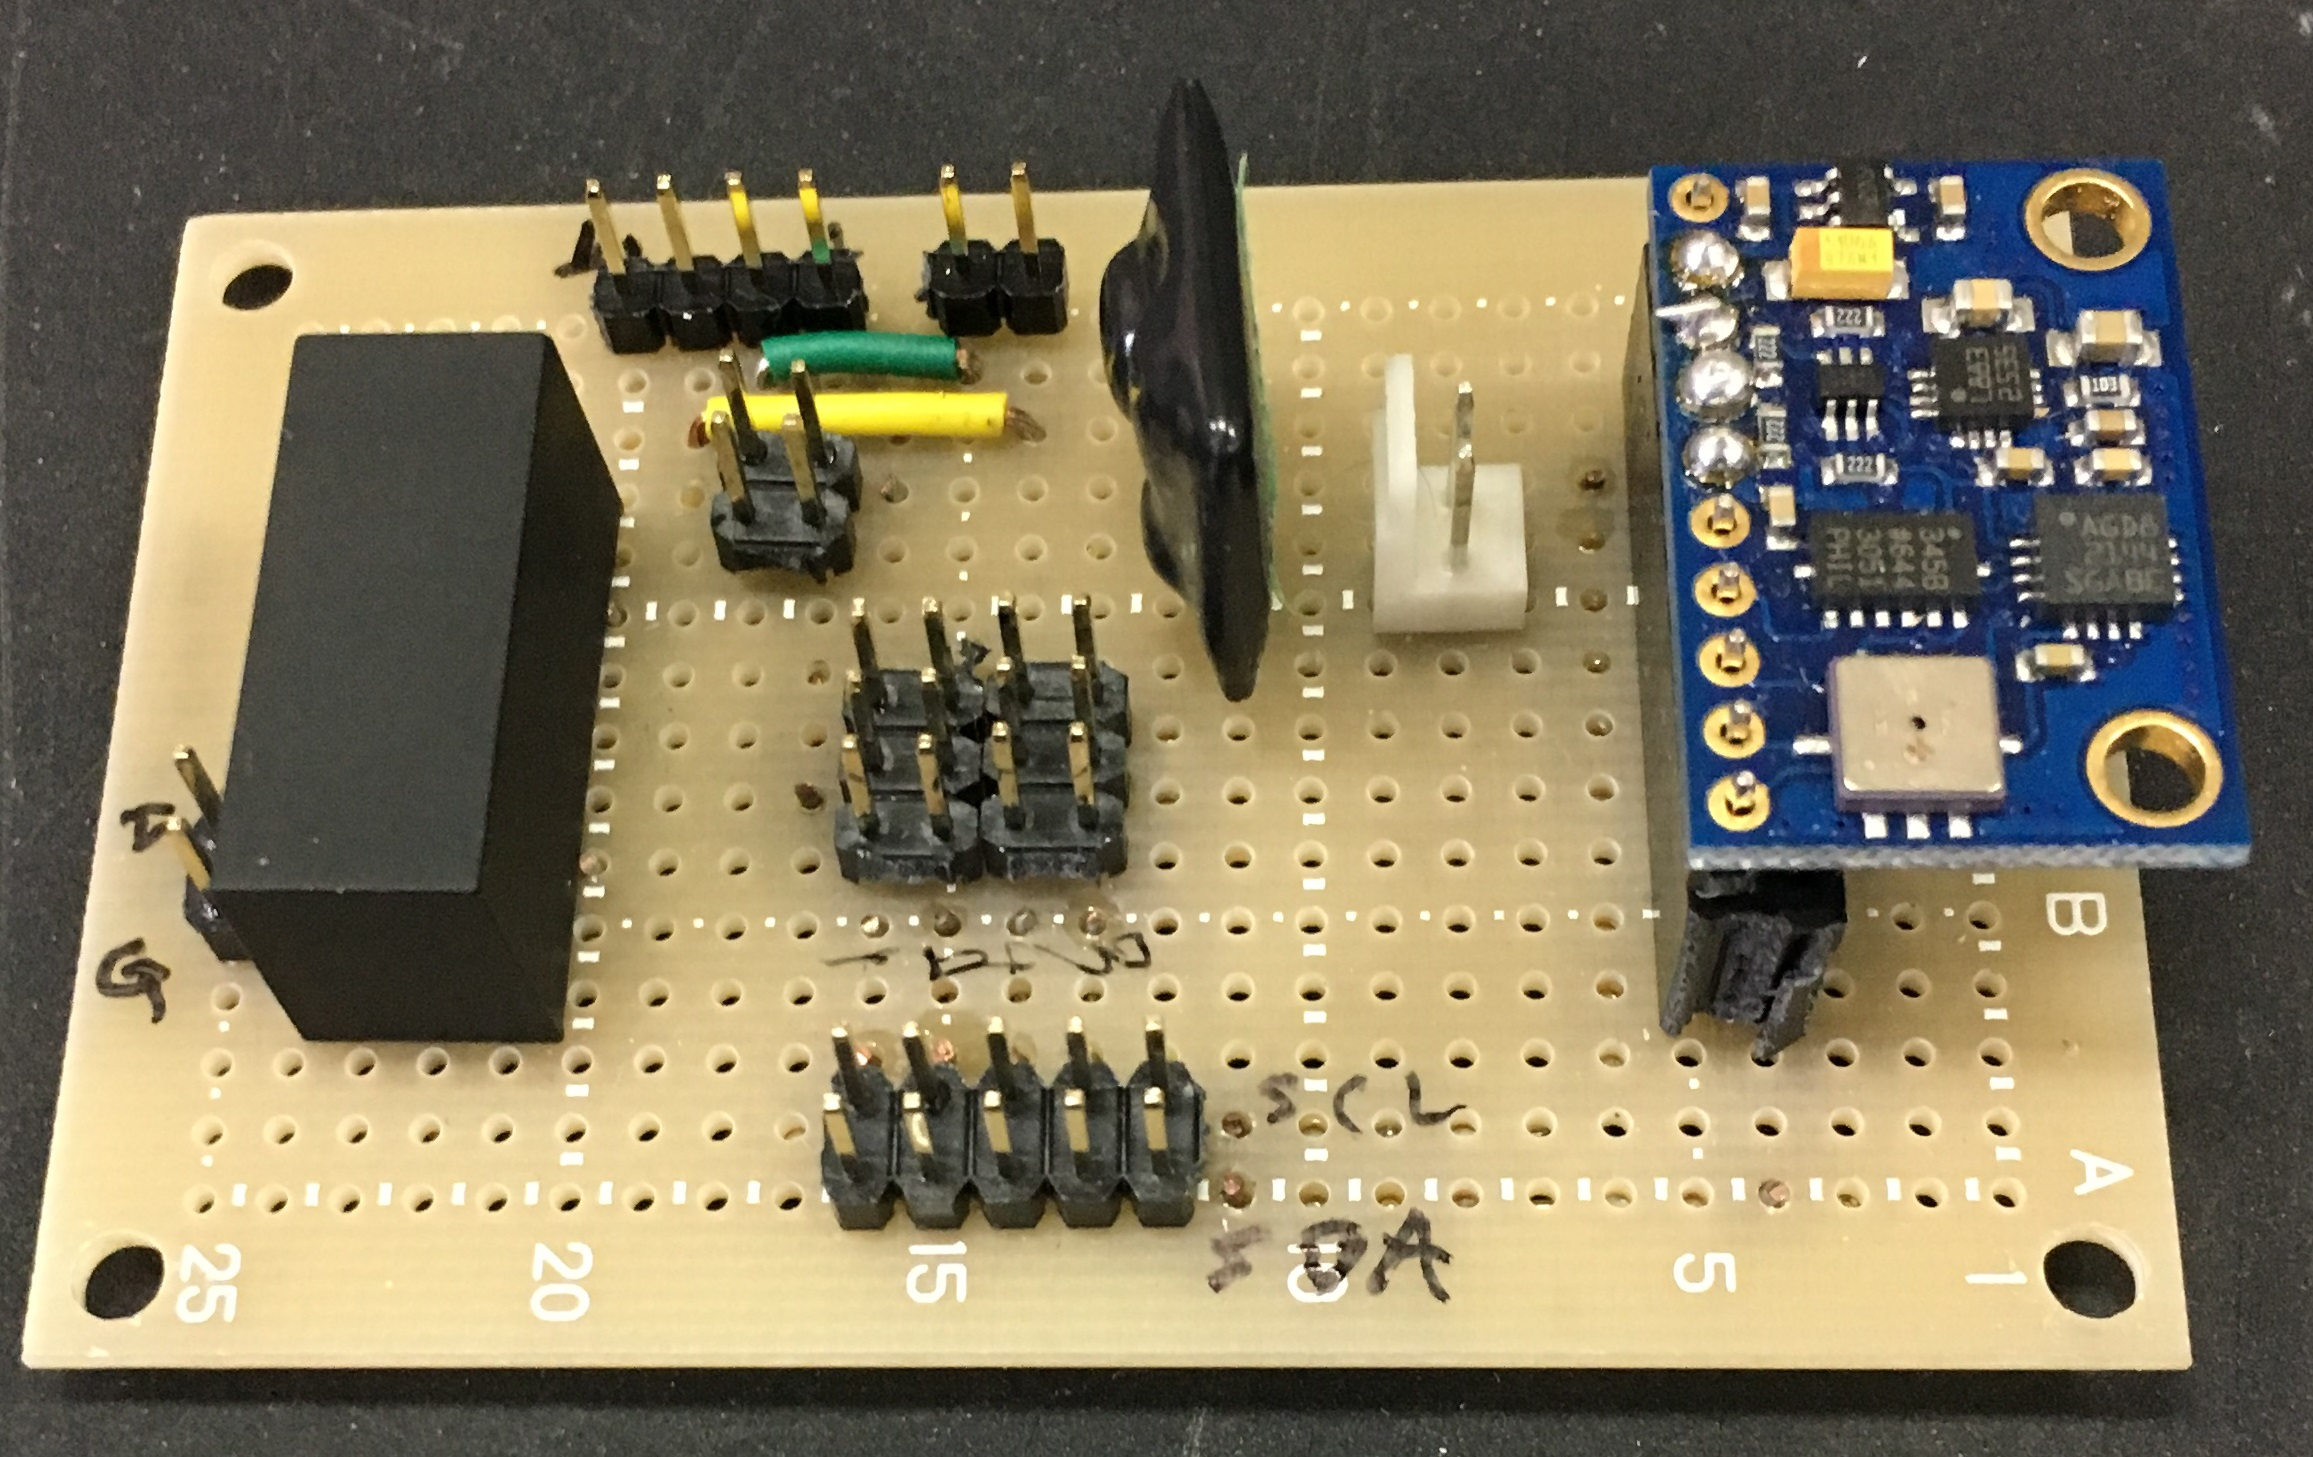
\includegraphics[width=90mm]{ga/kairo1.jpeg}
\end{center}
\caption{電子回路}
\label{fig:kairo}
\end{figure}

フレームに使用電子部品を配置した自作ドローンの完成図が以下の図\ref{fig:erc}となる.

\begin{figure}[H]
\begin{center}
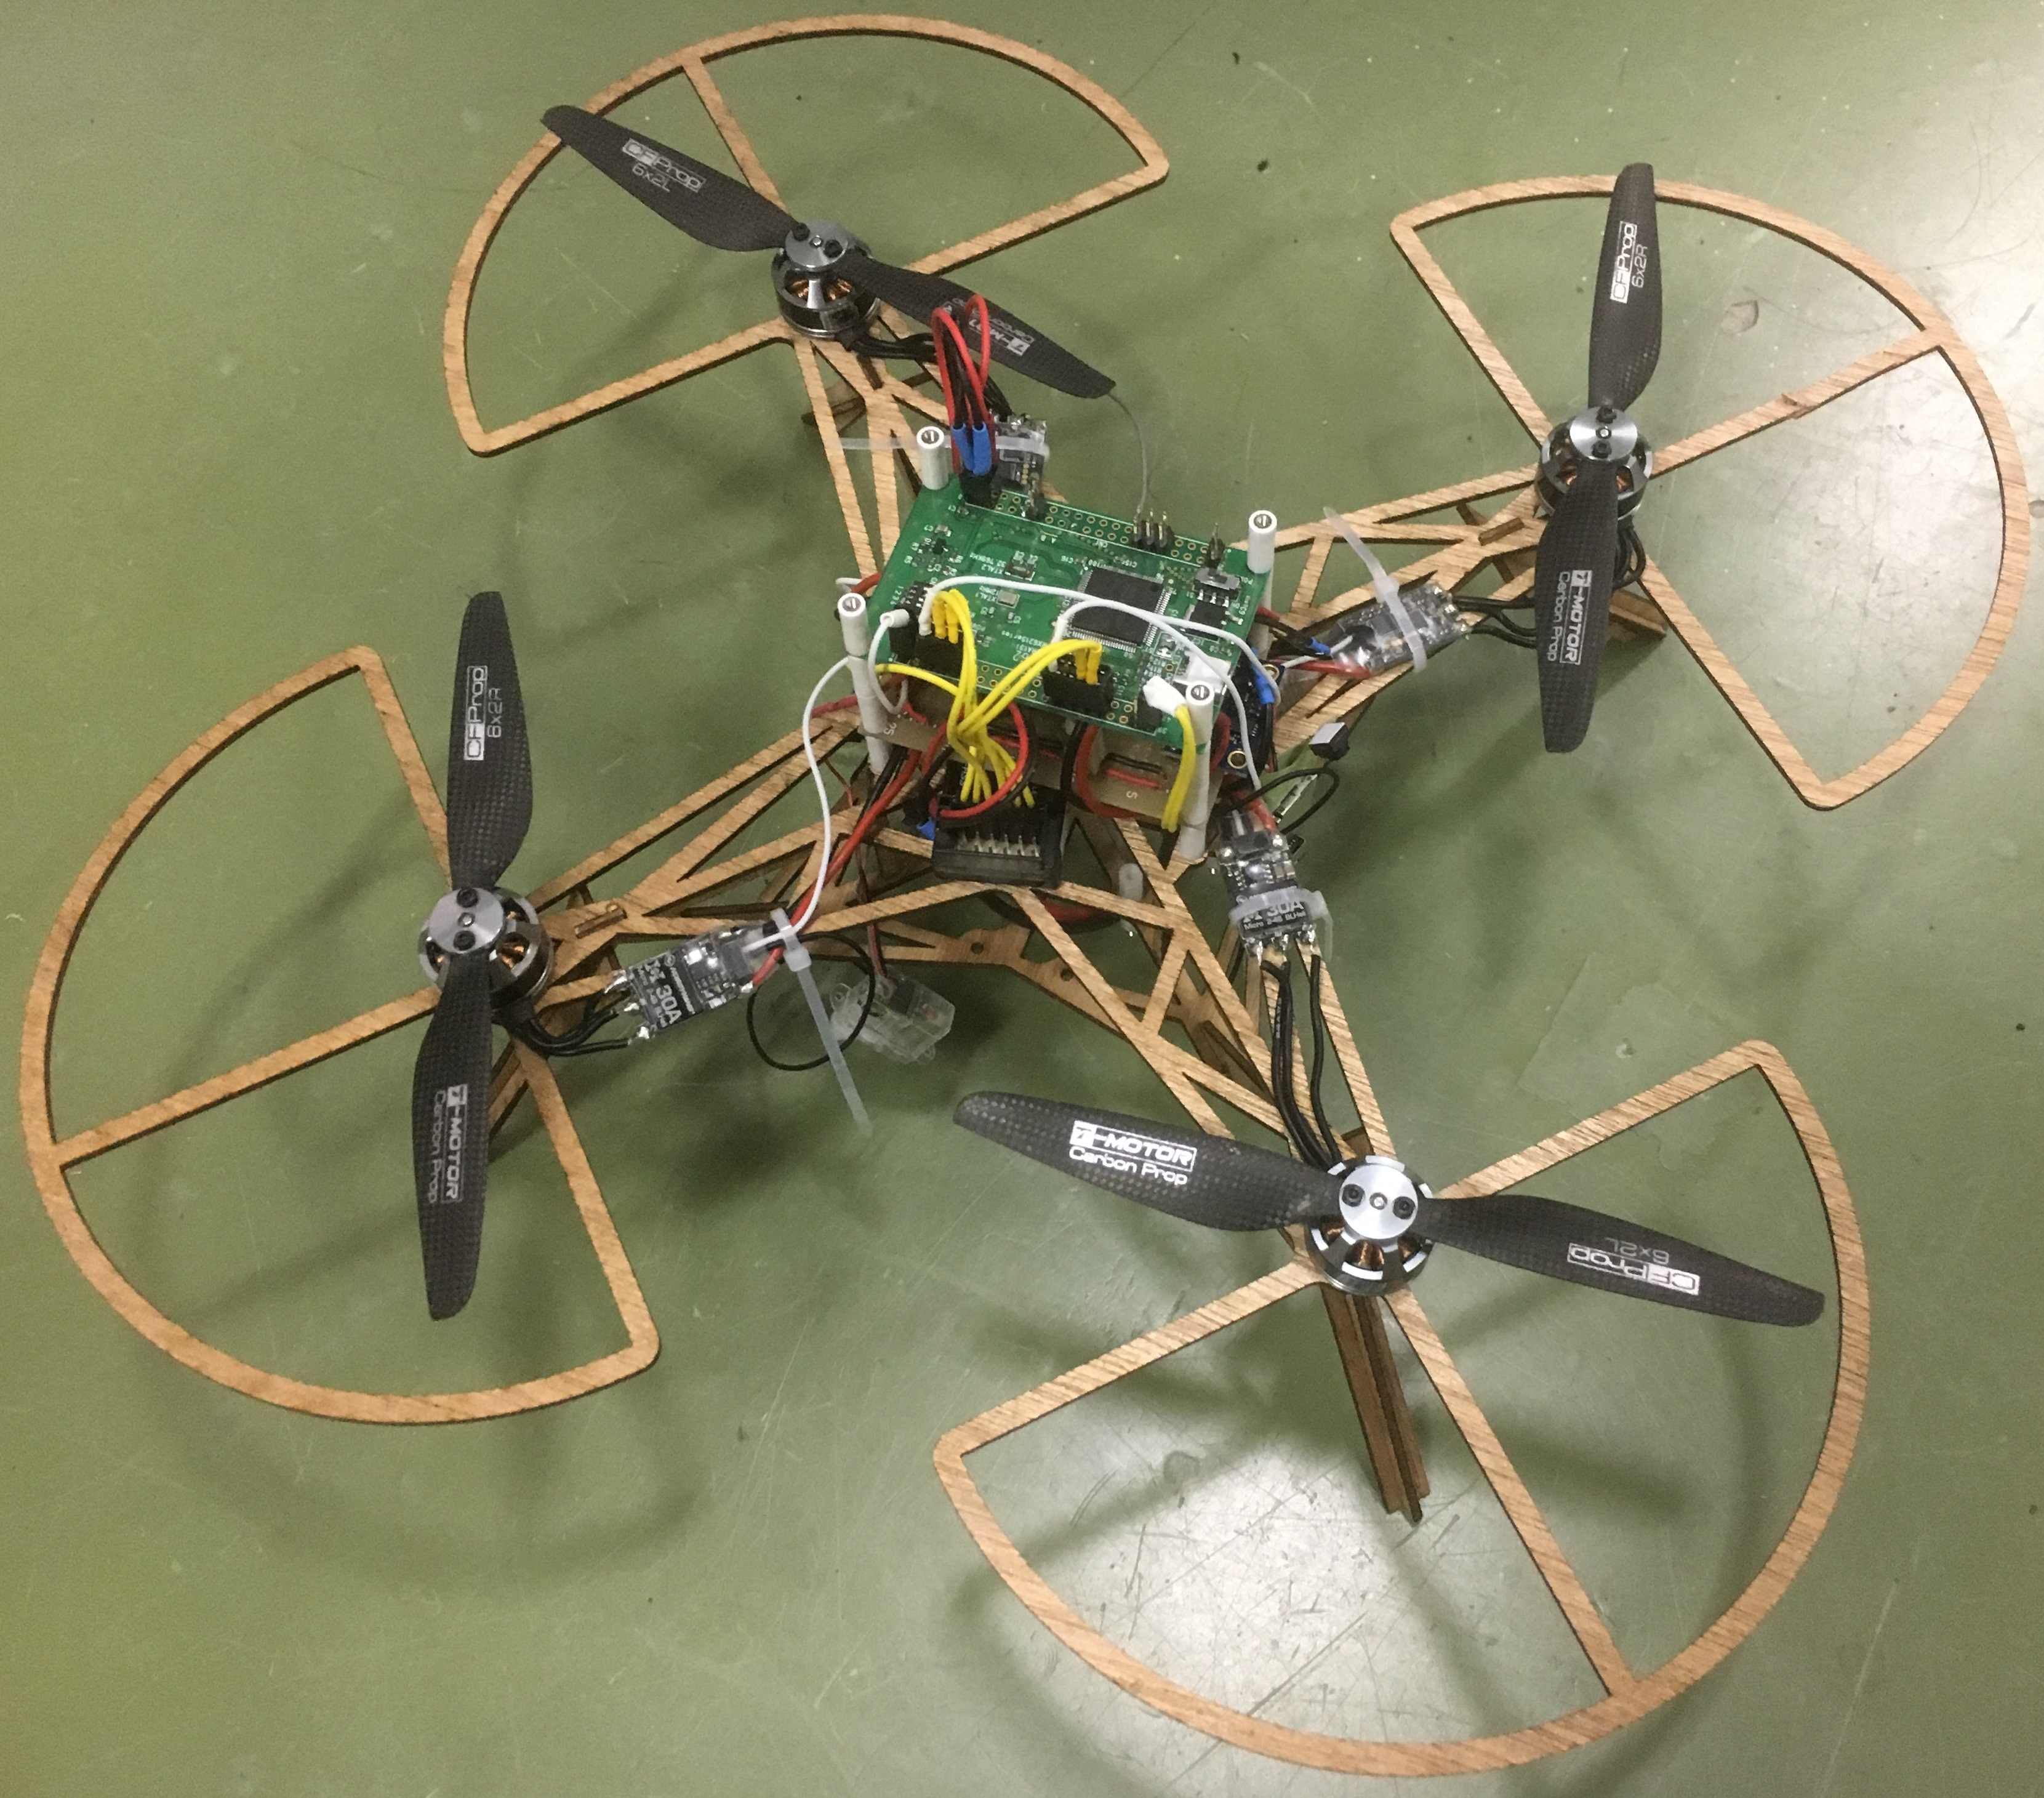
\includegraphics[width=90mm]{ga/erc.jpg}
\end{center}
\caption{自作ドローン完成図}
\label{fig:erc}
\end{figure}

\section{使用するマイコンの機能}今回使用したマイコンに含まれている機能は以下のようになっている.

\subsection{マルチファンクションタイマパルスユニット 2(MTU2)}受信機から送られる信号をこの機能で処理することによってESCへと信号を送り,モーターを制御する.

この機能を使用するためには,使用する送信機のパルス幅をオシロスコープ等で測り,プログラムで書き込む必要があり,更に割り込みというある時間や条件がそろうと今読み込んでいるプログラムの読込みを中断し,別のプログラムを読み込むといった動作がありそのプログラムとのかみ合いをそろえたりするのに苦労した.だが,設定はややこしいもののプログラムの設定さえ間違っていなければ問題なくこなせるものでもある.

\subsection{I2C バスインタフェース(RIIC)}この機能はマイコンがI2C通信をするための機能で,マイコン側のI2C通信の設定,ジャイロセンサとデータのやり取りをするために使用される.

\section{ジャイロセンサ}主に市販で売られているドローンや自作で製作するときに使われているマイコンはフライトコントローラーと呼ばれるジャイロセンサ,加速度センサ,気圧センサ,GPSといった機体の姿勢を制御し安定させるセンサーを含んだコンピューターを使用しドローンを制御するのだが,今回はマイコンとセンサーを別々にし,シリアル通信を利用してセンサーから来るデータのやり取りを行った.


\chapter{ジャイロセンサとマイコン間の通信}

\section{通信方法}ジャイロセンサとマイコンとのデータのやり取りはI2C通信を使用しデータ通信を行う.
 

\subsection{I2C通信とは}I2C(Inter-Integrated Circuit)とは,フィリップス社が開発した複数のデバイスとシリアル通信を行う通信方法の1つである.
この通信方法の大きな特徴はデータ通信のすべての権限を持つデバイス(マスタ)とそれ以外のデバイス(スレーブ)間で2本の信号線SDA(シリアルデータ)とSCL(シリアルクロック)でマスタとスレーブ間のデータ通信を行う.ここでのマスタ側のデバイスはマイコンで,スレーブ側をジャイロセンサとする.この関係図を図 \ref{fig:i2c} に示す.

\begin{figure}[H]
  \begin{center}
    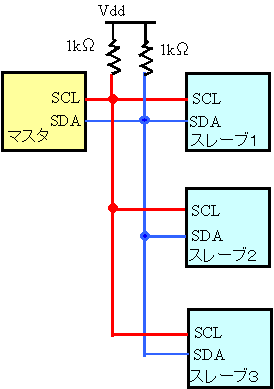
\includegraphics[width=60mm]{ga/i2c.png}
    \end{center}
  \caption{I2C通信}
 \label{fig:i2c}
\end{figure}

\subsubsection{SCLとSDA}
図 \ref{fig:i2c}にあるSCLはスレーブとの同期をとるための信号線で,通常はマスターからスレーブへの一方通行の線である.
一方,SDAはSCLに同期し,データの転送に用いる信号線であり,マスターとスレーブ,どちらからも送信される.


\subsubsection{書込みの流れ}

マスタ側からスタートコンディションを発行し通信を開始したら,マスタ側から''通信するスレーブ''と''マスタ側が書込み''アドレスを8bit分送信しスレーブ側から正常に送信されたことを意味するACKという1bit分のデータが返される.この次からスレーブに書き込みたいデータを約1byte分送りACKがスレーブから送られる.そしてすべてのデータの送信が終了したら,ストップコンディションを発行し通信を終える.

\begin{figure}[htbp]
  \begin{center}
    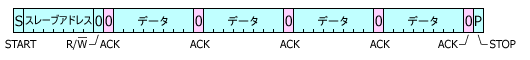
\includegraphics[width=100mm]{ga/i2c_w.png}
    \end{center}
  \caption{I2C書込み}
 \label{fig:i2c_w}
\end{figure}

\subsubsection{読込みの流れ}

マスタ側からスタートコンディションを発行し通信を開始したら,マスタ側から''通信するスレーブ''と''マスタ側が読込む''アドレスを8bit分送信しスレーブ側からACKが返される.そしてスレーブから送られるデータを約1byte分もらい,ACKをスレーブに送る.そしてすべてのデータの送信が終了したら,ストップコンディションを発行し通信を終える.

\begin{figure}[H]
  \begin{center}
    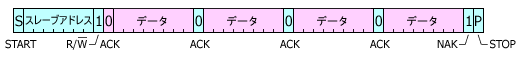
\includegraphics[width=100mm]{ga/i2c_r.png}
    \end{center}
  \caption{I2C読込み}
 \label{fig:i2c_r}
\end{figure}

\subsection{通信方法}通信プログラムの流れはジャイロセンサーのマニュアルの方法で図\ref{fig:flo}のようなフローチャートとなる.
マニュアルより,図\ref{fig:gyro_m}の流れは図\ref{fig:flo}の所の'ステータスレジスタのアドレスを送る'の所から'データをもらう'までの部分となる.

\begin{figure}[H]
  \begin{center}
    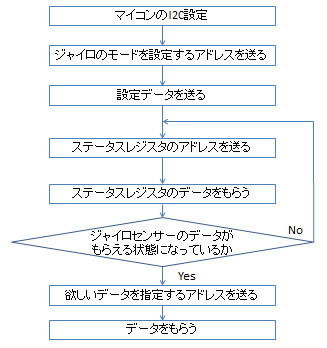
\includegraphics[width=80mm]{ga/flo.png}
    \end{center}
  \caption{通信フローチャート}
 \label{fig:flo}
\end{figure}

\begin{figure}[H]
  \begin{center}
    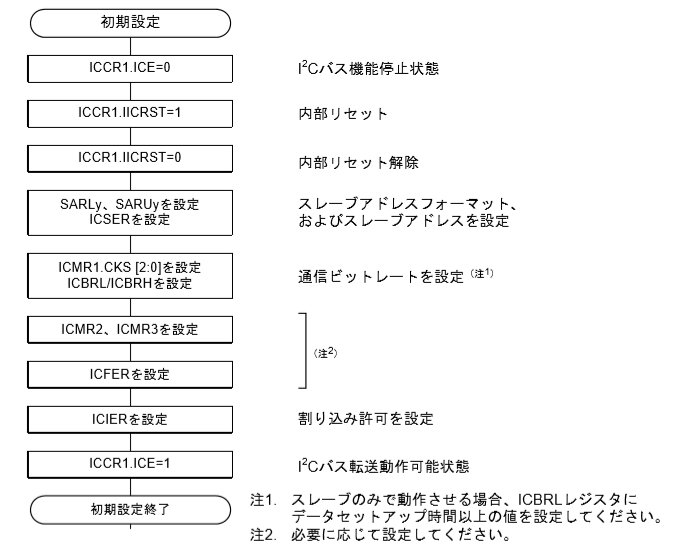
\includegraphics[width=100mm]{ga/rx_set.png}
    \end{center}
  \caption{マイコンのI2C通信設定手順}
 \label{fig:rx_set}
\end{figure}

\begin{figure}[H]
  \begin{center}
    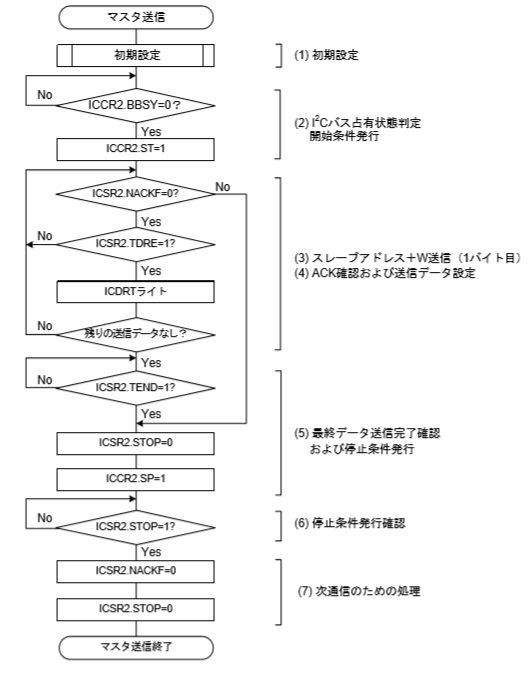
\includegraphics[width=100mm]{ga/rx_w.png}
    \end{center}
  \caption{I2C通信,送信時プログラミング手順}
 \label{fig:rx_w}
\end{figure}


\begin{figure}[H]
  \begin{center}
    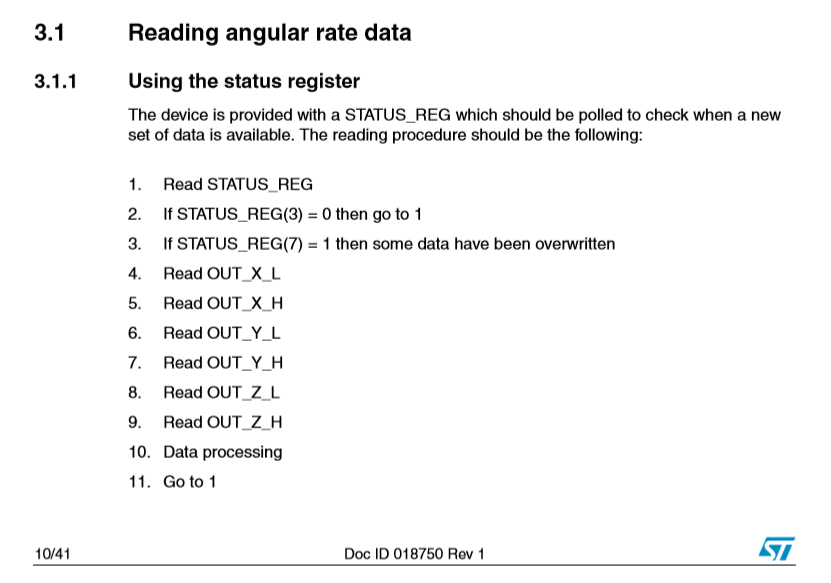
\includegraphics[width=100mm]{ga/gyro_m.png}
    \end{center}
  \caption{ジャイロセンサーのデータ受信手順}
 \label{fig:gyro_m}
\end{figure}

始めにマイコン側で通信速度や使用するレジスタの設定を行いジャイロセンサーを起動させるために,書込みでジャイロの設定するレジスタのアドレスを送り起動するようにと設定を通信で書き換える.
次にジャイロが起動しているかを調べるために読込みでステータスレジスタのデータをもらうことによって起動しているかどうかを調べる.ここでジャイロが起動していなければ,もう一度調べるところから戻る.
無事起動できていれば,ジャイロの欲しいデータがあるレジスタを書込みでアドレスを送り,指定したのち,読込みでデータをもらう.
なお,ジャイロからもらうデータはX軸Y軸Z軸の上位と下位それぞれ8bitずつに分けられた6つのデータをもらう.

\subsection{プログラム製作}製作した主な関数の大まかな流れが以下のようになり,それぞれ使用する関数の説明を次に説明する.

\begin{figure}[H]
  \begin{center}
    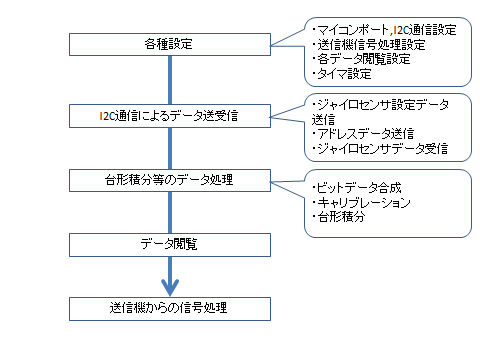
\includegraphics[width=100mm]{ga/kanflo.png}
    \end{center}
  \caption{使用関数フローチャート}
 \label{fig:kanflo}
\end{figure}

\subsubsection{メイン}
\begin{enumerate}
\item 関数名:main()
\item 機能:ここで各関数の処理を行う.
\item 引数:なし
\item 戻り値:なし
\end{enumerate}

\subsubsection{マイコンポート設定}

\begin{enumerate}
\item 関数名:i2c\_portset()
\item 機能:マイコンで使用するポートを起動する.
\item 引数:なし
\item 戻り値:なし
\end{enumerate}

\subsubsection{マイコンI2C通信設定}

\begin{enumerate}
\item 関数名:i2c\_set()
\item 機能:I2C通信の通信速度等の設定.マイコンマニュアルのRIIC0の説明をもとに通信するデバイスに合わせた設定をする.
\item 引数:なし
\item 戻り値:なし
\end{enumerate}

\subsubsection{送信機信号処理設定}

\begin{enumerate}
\item 関数名:receiver\_main()
\item 機能:送信機の信号処理に必要なマイコン内のMTU機能,PWM機能の設定.
\item 引数:なし
\item 戻り値:なし
\end{enumerate}

\subsubsection{各データ閲覧設定}

\begin{enumerate}
\item 関数名:init\_serial()
\item 機能:シリアル通信を利用し,パソコンでジャイロセンサのデータを見れるようにするための設定.
\item 引数:なし
\item 戻り値:なし
\end{enumerate}

\subsubsection{タイマ設定}

\begin{enumerate}
\item 関数名:time\_CMT0()
\item 機能:一定時間ごとにジャイロセンサのデータを貰えるようにする.CKSとCMCORのビットでデータを貰う速度を変えられる.
\item 引数:なし
\item 戻り値:なし
\end{enumerate}

\subsubsection{ジャイロセンサ設定データ送信}

\begin{enumerate}
\item 関数名:gyro\_set()
\item 機能:ジャイロセンサが測定する軸等の設定をI2C通信のデータ送信を利用して設定する.今回は特に複数のデータを送るわけではないため引数は使わず直接データ等を打ち込んでいる.
\item 引数:なし
\item 戻り値:なし
\end{enumerate}

\subsubsection{アドレスデータ送信}

\begin{enumerate}
\item 関数名:write\_addr()
\item 機能:欲しいデータがあるデバイスにアドレスで指定する.引数にアドレスを書き込むことで,アドレスデータを送れる.
\item 引数:通信したいスレーブデバイスのアドレス
\item 戻り値:なし
\end{enumerate}

\subsubsection{ジャイロセンサデータ受信}

\begin{enumerate}
\item 関数名:read\_data()
\item 機能:指定したデバイスからデータを貰う.貰ったデータはreturnで引数に格納されることにより,X=read\_data()でデータを別の変数に書き込むことが可能.	
\item 引数:returnで返されたジャイロセンサのデータ.
\item 戻り値:ジャイロセンサから貰ったデータ.
\end{enumerate}

\subsubsection{ビットデータ合成}

\begin{enumerate}
\item 関数名: deta\_H\_ave(),deta\_HL()
\item 機能:上位8bitに265をかけ,下位8bitのデータと足し合わせることで1つの16bitのデータとなる.
\item 引数:X,Y,Zのhighとlowデータ
\item 戻り値:highとlowが1つとなったデータ
\end{enumerate}

\subsubsection{キャリブレーション}

\begin{enumerate}
\item 関数名:cya()
\item 機能:ジャイロセンサのデータを平均化させその値と比べることにより,角速度に近い値を出す.
\item 引数:なし
\item 戻り値:キャリブレーションデータ
\end{enumerate}

\subsubsection{台形積分}

\begin{enumerate}
\item 関数名:integral()
\item 機能:ビットデータ合成で得た角速度データをここで計算して,角度データにする.
\item 引数:ビットデータ合成で得た角速度データ.
\item 戻り値:積分結果.
\end{enumerate}

\subsubsection{送信機信号処理}

\begin{enumerate}
\item 関数名:receiver\_main\_while()
\item 機能:送信機からの信号を各ESCに送る信号へ処理する.
\item 引数:なし
\item 戻り値:なし
\end{enumerate}

\subsubsection{各データ閲覧}
\begin{enumerate}
\item 関数名:deta\_look(),deta\_cross(),serial()
\item 機能:ジャイロセンサから受け取ったデータや,マイコン内で処理しているデータを引数として関数に組み込むとデータが見れるようになる.deta\_look()でジャイロセンサからそのまま受け取ったデータ,deta\_cross()でビットデータ合成で得たデータ,serial()で台形積分した計算結果が閲覧できる.
\item 引数:それぞれのジャイロセンサのデータ.
\item 戻り値:なし
\end{enumerate}


\chapter{角速度及び角度の取得について}ここではドローンを飛ばすための制御プログラムについて説明する.

\section{MTU機能を利用したマルチコプタの方向転換方法}
受信機からマイコンへ送られる信号を図\ref{fig:mtu}インプットキャプチャで拾いTGRAとTGRBに反映し,これらの値を引くことによりパルス幅を作り出しESCへ,そのパルスを送る仕組みとなっている.


\begin{figure}[H]
  \begin{center}
    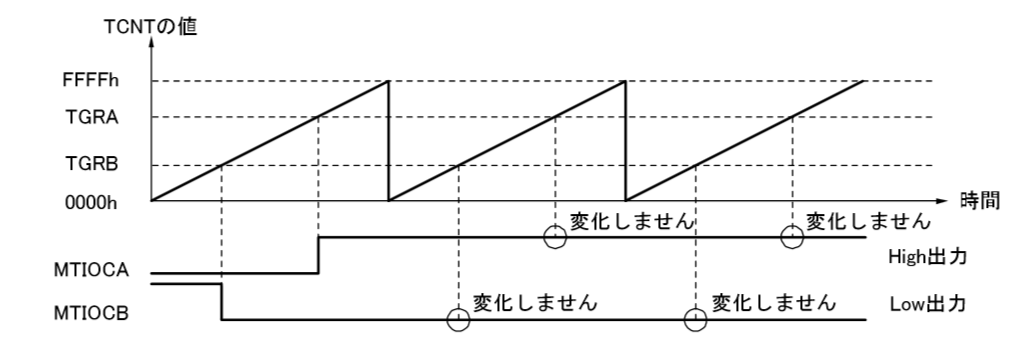
\includegraphics[width=100mm]{ga/mtu.png}
    \end{center}
  \caption{インプットキャプチャ}
 \label{fig:mtu}
\end{figure}

\section{角度推定方法}ジャイロから送られるデータは角度ではなく角速度である.よって,ジャイロから送られた角速度のデータを角度に変換する動作をプログラムにする必要がある.ここではその方法を説明する.

\subsection{データキャリブレーション}ただジャイロセンサーから取った値ではまだ使用できるものではなく,最初に図\ref{fig:rollcya}のように大体10000近くのデータを取得しそのデータを平均した値を制御に反映させるデータから引く動作が必要となる.これをキャリブレーションという.

\begin{figure}[H]
  \begin{center}
    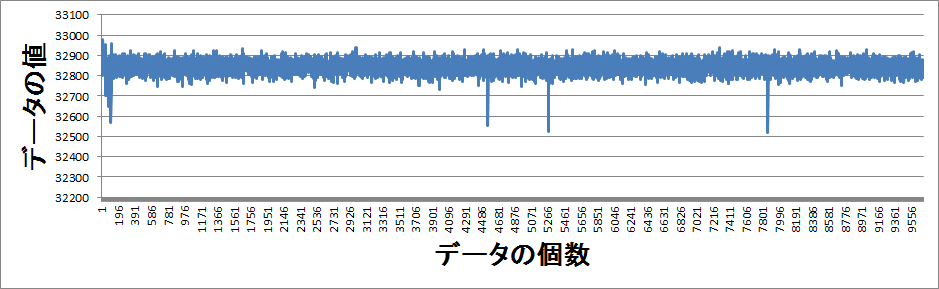
\includegraphics[width=110mm]{ga/rollcya.png}
    \end{center}
  \caption{キャリブレーション用データ}
 \label{fig:rollcya}
\end{figure}

\subsection{台形法での積分方法}ジャイロセンサーからもらえるデータはあくまで角速度のデータなので積分をして角度に直す必要がある.今回は台形法という定積分を近似計算する方法を使用し.常時値を足し合わせることによって角度を求める.使用する式は以下の式(\ref{siki1})となる.

\begin{eqnarray}
d=\Sigma \frac{(a+b)t}{2}
\label{siki1}
\end{eqnarray}

\begin{table}[H]
 \begin{center}
  \caption{文字意味}
   \begin{tabular}[htbp]{|c|c|}
    \hline
    d & 角度\\
    \hline
    a & ひとつ前のデータ\\
    \hline
    b & 新しいデータ\\
    \hline
    t & 時間\\
    \hline
   \end{tabular}
 \end{center}
\end{table}

\subsection{データを取った結果}
キャリブレーションで得たデータが以下の図\ref{fig:jiken_vero}となりそこから式(\ref{siki1})で計算し,でた値を図\ref{fig:jiken}に示す.

\begin{figure}[H]
  \begin{center}
    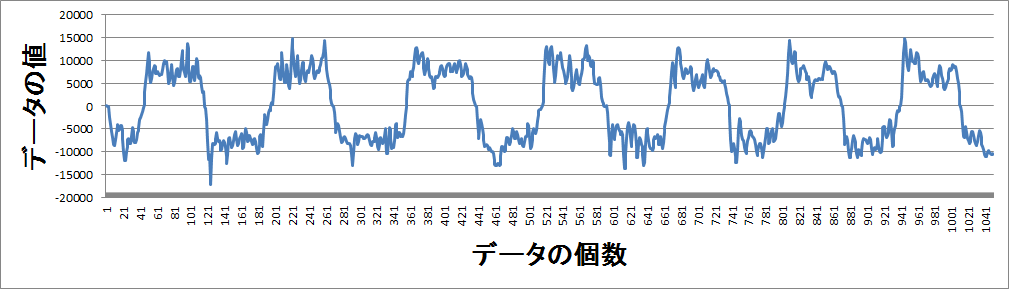
\includegraphics[width=110mm]{ga/jiken_vero.png}
    \end{center}
  \caption{キャリブレーションしたデータ}
 \label{fig:jiken_vero}
\end{figure}

\begin{figure}[H]
  \begin{center}
    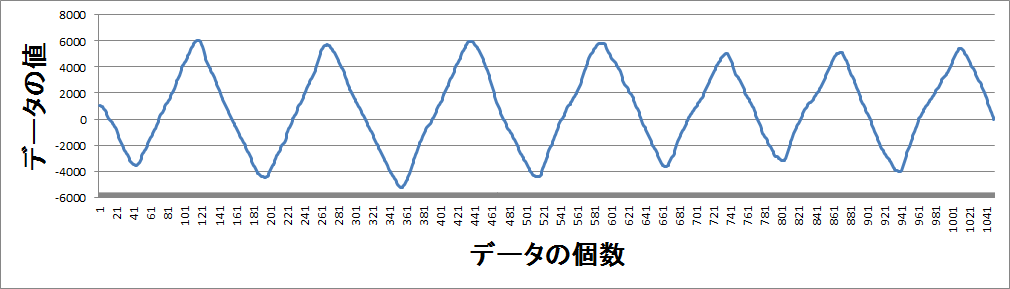
\includegraphics[width=110mm]{ga/jiken.png}
    \end{center}
  \caption{台形積分したデータ}
 \label{fig:jiken}
\end{figure}

しかし,これらの取得したデータは生データであって物理量ではないためこの角度のデータ量はどれほどの大きさなのかは不明である.
しかし,図\ref{fig:jiken}のデータの個数3400以降でセンサを1秒ごとに左右に30度ほど傾けた時のデータ値の揺れ幅の大きさが静止した時との差でどれ程の値の大きさなのかが分かる.


\section{フィードバック制御の流れ}
ジャイロセンサからもらったデータを処理しドローンの制御をするためにフィードバック制御のサイクルを使用しの図 \ref{fig:seigyo} となっている.

\begin{figure}[H]
  \begin{center}
    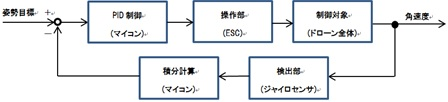
\includegraphics[width=100mm]{ga/seigyo.jpg}
    \end{center}
  \caption{フィードバック制御}
 \label{fig:seigyo}
\end{figure}


\chapter{結論}
\section{本研究のまとめ}データの取得及びまで至れたが,今だドローンを飛ばすまでには到達できていない.しかし,後は取得したデータをもとに角度を算出し,各ドローンの制御プログラムを合わせ,ジャイロセンサの値でモーターを制御するというところまで到達しているため,残りの時間の間この製作をしていく予定である.

\section{今後の課題}
センサを90度に傾けた時のデータとジャイロから得た生データを比べ,角度を算出する.
このデータをもとにして安定化制御を行う.


\begin{thebibliography}{8}
\bibitem{maikon} 新海栄治,石黒裕紀,伊藤彩子, 仲めぐみ,藤澤幸穂:RXマイコンのすべて,株式会社 電波新聞社,2012
\bibitem{i2c} I2C通信の使い方-電子工作の実験室,http://www.picfun.com/c15.html , 
\end{thebibliography}

\chapter*{謝辞}
\addcontentsline{toc}{chapter}{謝辞}
本論文作成にあたりテーマの決定,研究の考え方,方法のまとめ方など全てにおいて長期にわたって厳しくも熱意のあるご指導,ご鞭撻していただいた,伊藤恒平教授に厚く御礼申し上げます.


特に分析においても論文の書き方においても論文を何度も読んでいただき,指導していただいた伊藤恒平教授に大変ご苦労をかけてしまいましたことにも心よりお詫び申し上げたいです.


同級生のメンバーには論文の作成,修正にご協力いただき心より感謝しております.
その他、助けていただいた多くの皆様に心から感謝しております.ありがとうございました.

\appendix
\chapter{プログラム}

\lstinputlisting[caption=メイン関数(RX621),label=I2C]{prog/I2C.cpp}
\lstinputlisting[caption=マイコンポート設定(RX621),label=i2c_portset]{prog/i2c_portset.cpp}
\lstinputlisting[caption=ジャイロセンサ送受信プログラム(RX621),label=i2c_S_W_R]{prog/i2c_S_W_R.cpp}
%\lstinputlisting[caption=割込み関数プログラム(RX621),label=intprg]{prog/intprg.cpp}
\lstinputlisting[caption=ジャイロセンサデータ処理プログラム(RX621),label=read_xyz]{prog/read_xyz.cpp}
\lstinputlisting[caption=送信機信号処理プログラム(RX621),label=Receiver]{prog/Receiver.cpp}
\lstinputlisting[caption=データ閲覧プログラム(RX621),label=rxserial]{prog/rxserial.cpp}

\end{document}
htpb
